\documentclass[11pt,a4paper]{article}

% Typography & Layout.
\usepackage[utf8]{inputenc}
\usepackage[T1]{fontenc}
\usepackage{mathpazo}
\usepackage[margin=1.25in]{geometry}
\usepackage{titlesec}
\usepackage{setspace}
\usepackage{microtype}
\usepackage{enumitem}
\usepackage{amsmath}
\usepackage{amssymb}
\usepackage{amsthm}
\usepackage{caption}
\usepackage{tcolorbox}
\tcbuselibrary{skins, breakable}
\usepackage{tikz}
\usetikzlibrary{arrows.meta, calc, decorations.pathreplacing}

% Formatting.
\titleformat{\section}{\Large\bfseries}{\thesection}{1em}{}
\titleformat{\subsection}{\large\bfseries}{\thesubsection}{1em}{}
\onehalfspacing
\setlist[enumerate]{label=(\alph*), nosep}
\setlist[description]{leftmargin=1.5em, itemsep=0pt}
\captionsetup{font=small, labelfont=bf, labelsep=period, skip=6pt}

% Environments.
\newtheoremstyle{boxed}{0pt}{0pt}{\normalfont}{0pt}{\bfseries\color{mirrorc}}{}{\newline}{\thmname{#1}\thmnumber{ #2}\thmnote{ (#3)}}
\theoremstyle{boxed}
\newtheorem{problem}{Problem}
\tcolorboxenvironment{problem}{enhanced, colback=mirrorc!4, colframe=mirrorc!50, boxrule=0.5pt, arc=2pt, left=8pt, right=8pt, top=6pt, bottom=6pt, before skip=12pt, after skip=10pt}
\theoremstyle{definition}
\newtheorem{fact}{Fact}
\newtheorem{corollary}{Corollary}
\newtheorem*{remark}{Remark}
\newtheorem*{note}{Note}
\newenvironment{solution}{\begin{proof}[Solution]}{\end{proof}}
\newenvironment{plate}{\par\medskip\noindent\begin{minipage}{\linewidth}\centering}{\end{minipage}\par\medskip}

% Notation.
\newcommand{\R}{\mathbb{R}}
\newcommand{\E}{\mathbb{E}^2}
\newcommand{\ip}[2]{\langle #1, #2 \rangle}
\newcommand{\abs}[1]{\lvert #1 \rvert}
\newcommand{\id}{\mathrm{id}}
\DeclareMathOperator{\rot}{rot}

% Figures.
\colorlet{mirrorc}{blue!60!black}
\colorlet{imgc}{red!70!black}
\tikzset{
    >={Stealth[length=2.2mm]},
    pt/.style={circle, fill=black, inner sep=0pt, minimum size=4pt},
    ipt/.style={pt, fill=imgc},
    hollow/.style={circle, draw=black, fill=white, inner sep=0pt, minimum size=4pt},
    mirror/.style={thick, mirrorc},
    aux/.style={densely dashed, gray},
    vec/.style={->, thick},
    base/.style={gray!70},
}
\newcommand{\eqtick}[2]{\draw ($(#1)!0.5!(#2)!1.2mm!90:(#2)$) -- ($(#1)!0.5!(#2)!1.2mm!-90:(#2)$);}

% Document...
\begin{document}

\begin{center}
    \vspace*{2em}
    {\Huge \textbf{Some Problems}}\\[0.5em]
    {\Large \textit{On Euclidean Geometry}}\\[2em]

    {\large \textbf{Juan S. A. Siagian}}\\[0.5em]
    {\normalsize Bandung, Indonesia \hspace{0.5em} $\cdot$ \hspace{0.5em} \today}\\[3em]
\end{center}

\section*{1. Preliminaries}

\subsection*{1.1 Points and Vectors}
We work in $\R^2$, whose elements are called points or vectors depending on their role.\\
Below, $\boldsymbol{x}$, $\boldsymbol{y}$, $\boldsymbol{u}$ and $\boldsymbol{v}$ are \textbf{vectors} and $\boldsymbol{P}$ and $\boldsymbol{Q}$ are \textbf{points}.
\begin{description}
    \item[Operations] $(x_1,x_2)+(y_1,y_2)=(x_1+y_1,\,x_2+y_2)$ and $c\,(x_1,x_2)=(cx_1,\,cx_2)$.
    \item[Inner product] $\ip{x}{y}=x_1y_1+x_2y_2$.
    \item[Length] $\abs{x}=\sqrt{\ip{x}{x}}$.
    \item[Distance] $d(P,Q)=\abs{Q-P}$. With this distance, $\R^2$ is the Euclidean plane $\E$.
    \item[Parallel] $u,v\neq0$ and $v=tu$ for some $t\in\R$.
    \item[Same direction] $u,v\neq0$ and $v=tu$ for some $t>0$.
    \item[Orthogonal] $\ip{u}{v}=0$.
    \item[Perpendicular vector] $v^\perp=(-v_2,v_1)$ for $v=(v_1,v_2)$.
\end{description}

\begin{note}
\leavevmode
\begin{enumerate}[label=\arabic*.]
    \item Parallel and same direction differ only in the sign of $t$. \\
    Parallel vectors may point opposite ways. \\
    Vectors with the same direction may not.
    \item The vector $v^\perp$ is a specific vector orthogonal to $v$. \\
    Built by turning $v$ by $90^\circ$ counterclockwise.
\end{enumerate}
\end{note}

\subsection*{1.2 Lines}
Below, $\boldsymbol{P}$, $\boldsymbol{Q}$ and $\boldsymbol{R}$ are \textbf{points} and $\boldsymbol{v}$ is a \textbf{vector}.
\begin{description}
    \item[Span] $[v]=\{tv \mid t\in\R\}$.
    \item[Line] A set $P+[v]=\{P+tv \mid t\in\R\}$ with $v\neq0$. Since $P+[0]=\{P\}$ is a single point.
    \item[Direction vector] The vector $v$ in $P+[v]$.
    \item[Between] $Q$ lies between $P$ and $R$ if $Q=P+s(R-P)$ for some $s\in[0,1]$.
\end{description}

\subsection*{1.3 Maps}
Below, $\boldsymbol{S}$ and $\boldsymbol{T}$ are \textbf{maps} from $\E$ to $\E$, $\boldsymbol{w}$ is a \textbf{vector} and $\boldsymbol{X}$ and $\boldsymbol{Y}$ are \textbf{points}.
\begin{description}
    \item[Identity] $\id(X)=X$.
    \item[Composition] $(S\circ T)(X)=S(T(X))$, so $T$ acts first.
    \item[Inverse] $T^{-1}$ is the map with $T\circ T^{-1}=T^{-1}\circ T=\id$, when it exists.
    \item[Translation] $T_w(X)=X+w$.
    \item[Isometry] $T$ with $d(T(X),T(Y))=d(X,Y)$ for all $X$ and $Y$.
\end{description}

\begin{note}
\leavevmode
\begin{enumerate}[label=\arabic*.]
    \item $T_a\circ T_b=T_{a+b}$ for all vectors $a$ and $b$, and $T_0=\id$. So $T_w^{-1}=T_{-w}$.
    \item An isometry is injective, since $T(X)=T(Y)$ gives $d(X,Y)=0$.
    \item Reflections, rotations and glide reflections are defined in later sections.
\end{enumerate}
\end{note}

\subsection*{1.4 Two Facts}
We take for granted the Cauchy--Schwarz inequality $\abs{\ip{u}{v}}\le\abs{u}\abs{v}$. \\
With equality exactly when $u=0$, $v=0$, or $u$ and $v$ are parallel.

\begin{fact}[Triangle inequality]\label{f:triangle}
For all $u,v\in\R^2$ we have $\abs{u+v}\le\abs{u}+\abs{v}$.
Equality holds if and only if $u=0$, or $v=0$, or $u$ and $v$ have the same direction.
\end{fact}

\begin{proof}
\leavevmode\\
By Cauchy--Schwarz
\[
\abs{u+v}^2=\abs{u}^2+2\ip{u}{v}+\abs{v}^2\le\abs{u}^2+2\abs{u}\abs{v}+\abs{v}^2=(\abs{u}+\abs{v})^2.
\]
Equality holds exactly when $\ip{u}{v}=\abs{u}\abs{v}$, and this happens in the following cases.
\begin{itemize}[nosep]
    \item If $u=0$ or $v=0$, both sides are $0$.
    \item If $v=tu$ with $t>0$, then $\ip{u}{v}=t\abs{u}^2=\abs{u}\abs{v}$.
    \item Conversely, let $u,v\neq0$ with $\ip{u}{v}=\abs{u}\abs{v}$.\\
    By Cauchy--Schwarz $v=tu$ with $t\neq0$, and $t\abs{u}^2=\abs{t}\abs{u}^2$ forces $t>0$. \qedhere
\end{itemize}
\end{proof}

\begin{fact}[Re-anchoring a line]\label{f:anchor}
\leavevmode
\begin{enumerate}
    \item If $X\in P+[v]$ and $c\neq0$, then $P+[v]=X+[cv]$. \\
    In particular every line has a direction vector of length $1$.
    \item If $P+[v]=P'+[v']$, then $v'$ is a multiple of $v$. \\
    So any two direction vectors of a line are parallel.
\end{enumerate}
\end{fact}

\begin{proof}
\leavevmode
\begin{enumerate}
    \item Write $X=P+sv$.
    Then $P+tv=X+\tfrac{t-s}{c}(cv)$ and $X+r(cv)=P+(s+rc)v$. Which gives both inclusions.
    For the last claim take $X=P$ and $c=1/\abs{v}$.
    \item Both $P'$ and $P'+v'$ lie in $P+[v]$, say $P'=P+sv$ and $P'+v'=P+rv$. \\
    Subtracting gives $v'=(r-s)v$. \qedhere
\end{enumerate}
\end{proof}

\section*{2. Lines}

\begin{problem}[The line through two points]\label{p:two-points}
Let $P$ and $Q$ be distinct points.
\begin{enumerate}
    \item Show that $\ell=P+[Q-P]$ is a line containing $P$ and $Q$.
    \item Show that every line containing $P$ and $Q$ is equal to $\ell$.
\end{enumerate}
Hence exactly one line contains $P$ and $Q$. We call it the line $PQ$.
\end{problem}

\begin{solution}
\leavevmode
\begin{enumerate}
    \item $\ell$ is a line because $Q-P\neq0$, and it contains $P$ and $Q$ because
    \[
    P=P+0\cdot(Q-P) \qquad\text{and}\qquad Q=P+1\cdot(Q-P).
    \]
    \item Let $\ell'=X+[v]$ be a line containing $P$ and $Q$. Then
    \[
    P=X+s_1v \qquad\text{and}\qquad Q=X+s_2v
    \]
    for some $s_1,s_2\in\R$. Subtracting gives $Q-P=(s_2-s_1)v$, and $s_2\neq s_1$ because $Q\neq P$. We prove both inclusions.
    \begin{enumerate}[leftmargin=2.5em]
        \item[($\subseteq$)] Let $Y\in\ell$, so $Y=P+t(Q-P)$ for some $t$.\\
        Substituting $P=X+s_1v$ and $Q-P=(s_2-s_1)v$ gives
        \[
        Y=X+s_1v+t(s_2-s_1)v=X+\bigl(s_1+t(s_2-s_1)\bigr)v\in\ell'.
        \]
        \item[($\supseteq$)] Let $Y\in\ell'$, so $Y=X+rv$ for some $r$.\\
        Substituting $X=P-s_1v$ and $v=(Q-P)/(s_2-s_1)$ gives
        \[
        Y=P+(r-s_1)v=P+\frac{r-s_1}{s_2-s_1}(Q-P)\in\ell.
        \]
    \end{enumerate}
    Hence $\ell'=\ell$. \qedhere
\end{enumerate}
\end{solution}

\begin{plate}
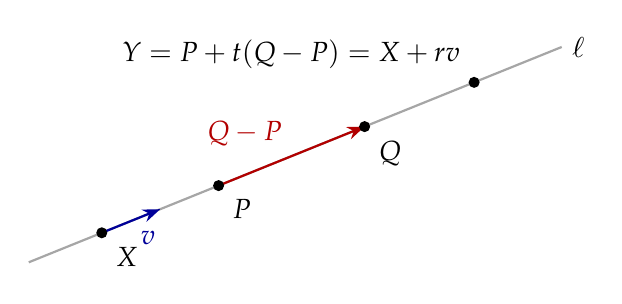
\begin{tikzpicture}
    \coordinate (P) at (0,0);
    \coordinate (Q) at (22:2);
    \coordinate (X) at (202:1.6);
    \coordinate (Y) at (22:3.5);
    \draw[base, thick] (202:2.6) -- (22:4.7) node[right, black] {$\ell$};
    \draw[vec, imgc] (P) -- (Q);
    \node[imgc, above left] at ($(P)!0.5!(Q)$) {$Q-P$};
    \draw[vec, mirrorc] (X) -- ($(X)+(22:0.8)$);
    \node[mirrorc, below right] at ($(X)+(22:0.4)$) {$v$};
    \node[pt, label=below right:{$P$}] at (P) {};
    \node[pt, label=below right:{$Q$}] at (Q) {};
    \node[pt, label=below right:{$X$}] at (X) {};
    \node[pt, label=above left:{$Y=P+t(Q-P)=X+rv$}] at (Y) {};
\end{tikzpicture}
\captionof{figure}{The line $\ell$ written as $P+[Q-P]$ and as $X+[v]$.}
\end{plate}

\newpage
\begin{problem}[Two lines meet at most once]\label{p:meet-once}
Show that two distinct lines have at most one point in common.
\end{problem}

\begin{solution}
\leavevmode\\
Suppose two distinct lines $\ell_1$ and $\ell_2$ share two distinct points $X$ and $Y$.\\
Applying Problem~\ref{p:two-points}(b) to each line gives $\ell_1=X+[Y-X]=\ell_2$.\\
This contradicts $\ell_1\neq\ell_2$.
\end{solution}

\begin{problem}[Betweenness and distance]\label{p:between}
Recall that a point $Q$ lies between $P$ and $R$ if $Q=P+s(R-P)$ for some $s\in[0,1]$.
Show that for all points $P$, $Q$ and $R$ the equation
\[
d(P,Q)+d(Q,R)=d(P,R)
\]
holds if and only if $Q$ lies between $P$ and $R$.
\end{problem}

\begin{solution}
\leavevmode\\
Put $u=R-Q$ and $v=Q-P$, so that $u+v=R-P$.\\
The equation then reads $\abs{u}+\abs{v}=\abs{u+v}$.
\begin{enumerate}[leftmargin=2.5em]
    \item[($\Rightarrow$)] By Fact~\ref{f:triangle} there are three cases.
    \begin{itemize}[nosep]
        \item $v=0$. Then $Q=P=P+0\cdot(R-P)$.
        \item $u=0$. Then $Q=R=P+1\cdot(R-P)$.
        \item $u=tv$ with $t>0$. Then $R-P=u+v=(1+t)(Q-P)$, so
        \[
        Q=P+s(R-P) \qquad\text{with}\qquad s=\frac{1}{1+t}.
        \]
        Since $t>0$ we have $1+t>1$, so $0<s<1$.
    \end{itemize}
    In every case $Q$ lies between $P$ and $R$.
    \item[($\Leftarrow$)] Let $Q=P+s(R-P)$ with $0\le s\le1$.\\
    Then $Q-P=s(R-P)$ and $R-Q=(1-s)(R-P)$, and since $s,\,1-s\ge0$
    \[
    d(P,Q)+d(Q,R)=s\abs{R-P}+(1-s)\abs{R-P}=\abs{R-P}=d(P,R). \qedhere
    \]
\end{enumerate}
\end{solution}

\begin{plate}
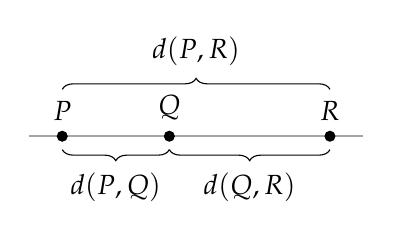
\begin{tikzpicture}[scale=0.85]
    \coordinate (P) at (0,0);
    \coordinate (Q) at (1.6,0);
    \coordinate (R) at (4,0);
    \draw[base, thick] (-0.5,0) -- (4.5,0);
    \draw[decorate, decoration={brace, mirror, amplitude=4pt}] (0,-0.2) -- (1.6,-0.2) node[midway, below=5pt] {$d(P,Q)$};
    \draw[decorate, decoration={brace, mirror, amplitude=4pt}] (1.6,-0.2) -- (4,-0.2) node[midway, below=5pt] {$d(Q,R)$};
    \draw[decorate, decoration={brace, amplitude=4pt}] (0,0.7) -- (4,0.7) node[midway, above=5pt] {$d(P,R)$};
    \node[pt, label=above:{$P$}] at (P) {};
    \node[pt, label=above:{$Q$}] at (Q) {};
    \node[pt, label=above:{$R$}] at (R) {};
\end{tikzpicture}
\hspace{1.5cm}
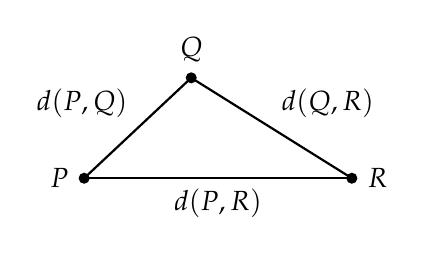
\begin{tikzpicture}[scale=0.85]
    \coordinate (P) at (0,0);
    \coordinate (Q) at (1.6,1.5);
    \coordinate (R) at (4,0);
    \draw[thick] (P) -- (Q) node[midway, above left] {$d(P,Q)$};
    \draw[thick] (Q) -- (R) node[midway, above right] {$d(Q,R)$};
    \draw[thick] (P) -- (R) node[midway, below] {$d(P,R)$};
    \node[pt, label=left:{$P$}] at (P) {};
    \node[pt, label=above:{$Q$}] at (Q) {};
    \node[pt, label=right:{$R$}] at (R) {};
\end{tikzpicture}
\captionof{figure}{Left, $Q$ lies between $P$ and $R$. Right, $Q$ is off the segment.}
\end{plate}

\begin{problem}[Reading the parameter from distances]\label{p:parameter}
Let $P\neq Q$ and let $X=(1-\lambda)P+\lambda Q$ for some $\lambda\in\R$.
\begin{enumerate}
    \item Show that
    \[
    \lambda=\frac{d(P,X)^2+d(P,Q)^2-d(Q,X)^2}{2\,d(P,Q)^2}.
    \]
    \item Deduce that a point on $PQ$ is determined by its distances to $P$ and $Q$.\\
    That is, for points $X$ and $X'$ on the line $PQ$
    \[
    d(P,X)=d(P,X') \ \text{and}\ d(Q,X)=d(Q,X') \implies X=X'.
    \]
\end{enumerate}
\end{problem}

\begin{solution}
\leavevmode
\begin{enumerate}
    \item From $X=(1-\lambda)P+\lambda Q$ we get $X-P=\lambda(Q-P)$.\\
    Writing $X-Q=(X-P)-(Q-P)$ and expanding the inner product gives
    \begin{align*}
    \abs{X-Q}^2 &= \abs{X-P}^2-2\ip{X-P}{Q-P}+\abs{Q-P}^2\\
    &= \abs{X-P}^2-2\lambda\abs{Q-P}^2+\abs{Q-P}^2.
    \end{align*}
    Since $P\neq Q$ we have $\abs{Q-P}^2\neq0$, so we can solve for $\lambda$.
    \[
    \lambda=\frac{\abs{X-P}^2+\abs{Q-P}^2-\abs{X-Q}^2}{2\abs{Q-P}^2}=\frac{d(P,X)^2+d(P,Q)^2-d(Q,X)^2}{2\,d(P,Q)^2}.
    \]
    \item By Problem~\ref{p:two-points} the line $PQ$ is $P+[Q-P]$, so
    \[
    X=(1-\lambda)P+\lambda Q \qquad\text{and}\qquad X'=(1-\lambda')P+\lambda'Q
    \]
    for some $\lambda,\lambda'\in\R$.\\
    By (a), $\lambda$ and $\lambda'$ come from the same formula in $d(P,\cdot)$, $d(Q,\cdot)$ and $d(P,Q)$.\\
    These distances agree for $X$ and $X'$, so $\lambda=\lambda'$ and $X=X'$.\\
    In Figure~\ref{fig:circles}, each circle meets $PQ$ twice and only $X$ lies on both. \qedhere
\end{enumerate}
\end{solution}

\begin{plate}
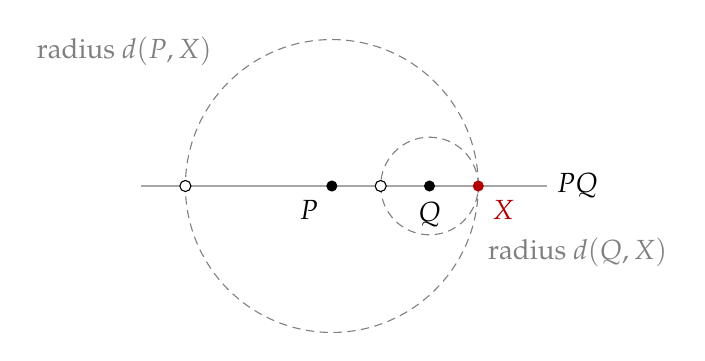
\begin{tikzpicture}[scale=0.62]
    \draw[base, thick] (-3.9,0) -- (4.4,0) node[right, black] {$PQ$};
    \draw[aux] (0,0) circle (3);
    \draw[aux] (2,0) circle (1);
    \node[hollow] at (-3,0) {};
    \node[hollow] at (1,0) {};
    \node[pt, label=below left:{$P$}] at (0,0) {};
    \node[pt, label=below:{$Q$}] at (2,0) {};
    \node[ipt, label={[imgc]below right:{$X$}}] at (3,0) {};
    \node[gray, anchor=south east] at (135:3.2) {radius $d(P,X)$};
    \node[gray, anchor=west] at (3.0,-1.35) {radius $d(Q,X)$};
\end{tikzpicture}
\captionof{figure}{The circles about $P$ and $Q$ through $X$, and the line $PQ$.}\label{fig:circles}
\end{plate}

\begin{problem}[Orthonormal coordinates]\label{p:orthonormal}
A pair $\{v,w\}$ of vectors is \emph{orthonormal} if $\abs{v}=\abs{w}=1$ and $\ip{v}{w}=0$.\\
Let $\{v,w\}$ be orthonormal.
\begin{enumerate}
    \item Show that $v$ and $w$ are linearly independent.
    \item Show that every $x\in\R^2$ satisfies $x=\ip{x}{v}v+\ip{x}{w}w$.
\end{enumerate}
\end{problem}

\begin{solution}
\leavevmode
\begin{enumerate}
    \item Suppose $av+bw=0$ for some $a,b\in\R$.\\
    Take the inner product with $v$ and with $w$.\\
    Since $\ip{v}{v}=\ip{w}{w}=1$ and $\ip{v}{w}=0$ this gives
    \begin{align*}
    0 &= \ip{av+bw}{v}=a\ip{v}{v}+b\ip{w}{v}=a\\
    0 &= \ip{av+bw}{w}=a\ip{v}{w}+b\ip{w}{w}=b.
    \end{align*}
    Hence $a=b=0$, so $v$ and $w$ are linearly independent.
    \item By (a), $v$ and $w$ are two independent vectors in the two-dimensional space $\R^2$.\\
    So they form a basis, and $x=x_1v+x_2w$ for some $x_1,x_2\in\R$.\\
    Taking inner products as in (a) gives
    \begin{align*}
    \ip{x}{v} &= x_1\ip{v}{v}+x_2\ip{w}{v}=x_1\\
    \ip{x}{w} &= x_1\ip{v}{w}+x_2\ip{w}{w}=x_2.
    \end{align*}
    Hence $x=\ip{x}{v}v+\ip{x}{w}w$.\\
    In Figure~\ref{fig:orthonormal}, these are the coordinates of $x$ along the turned axes $v$ and $w$. \qedhere
\end{enumerate}
\end{solution}

\begin{plate}
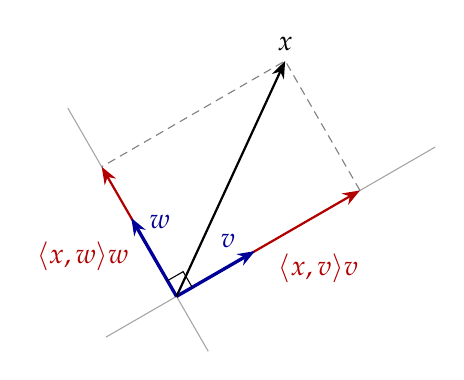
\begin{tikzpicture}[scale=1.15]
    \coordinate (O) at (0,0);
    \coordinate (A) at (30:2.339);
    \coordinate (B) at (120:1.652);
    \coordinate (X) at ($(A)+(B)$);
    \draw[base] (210:0.9) -- (30:3.3);
    \draw[base] (300:0.7) -- (120:2.4);
    \draw[aux] (A) -- (X) -- (B);
    \draw[vec, imgc] (O) -- (A) node[midway, below right] {$\ip{x}{v}v$};
    \draw[vec, imgc] (O) -- (B) node[midway, below left] {$\ip{x}{w}w$};
    \draw[vec, mirrorc, very thick] (O) -- (30:1);
    \draw[vec, mirrorc, very thick] (O) -- (120:1);
    \node[mirrorc] at ($(30:0.8)+(120:0.25)$) {$v$};
    \node[mirrorc] at ($(120:0.8)+(30:0.25)$) {$w$};
    \draw[vec] (O) -- (X) node[above] {$x$};
    \draw (30:0.2) -- ($(30:0.2)+(120:0.2)$) -- (120:0.2);
\end{tikzpicture}
\captionof{figure}{The vector $x$ and its components along an orthonormal pair $v$, $w$.}\label{fig:orthonormal}
\end{plate}

\begin{problem}[The perpendicular vector and the normal form of a line]\label{p:normal}
For $v=(v_1,v_2)$ let $v^\perp=(-v_2,v_1)$.
\begin{enumerate}
    \item Show that $\ip{v}{v^\perp}=0$ and $\abs{v^\perp}=\abs{v}$ for every $v$.\\
    Deduce that $\{v,v^\perp\}$ is orthonormal whenever $\abs{v}=1$.
    \item Let $P$ be a point and $v$ a unit vector. Show that
    \[
    P+[v]=\{X\in\E \mid \ip{X-P}{v^\perp}=0\}.
    \]
\end{enumerate}
\end{problem}

\begin{solution}
\leavevmode
\begin{enumerate}
    \item A direct computation gives
    \begin{align*}
    \ip{v}{v^\perp} &= v_1(-v_2)+v_2v_1=0\\
    \abs{v^\perp}^2 &= (-v_2)^2+v_1^2=\abs{v}^2.
    \end{align*}
    If $\abs{v}=1$, then also $\abs{v^\perp}=1$, so $\{v,v^\perp\}$ is orthonormal.
    \item We prove both inclusions.
    \begin{enumerate}[leftmargin=2.5em]
        \item[($\subseteq$)] Let $X=P+tv$ for some $t$.\\
        By (a), $\ip{X-P}{v^\perp}=t\ip{v}{v^\perp}=0$.
        \item[($\supseteq$)] Let $\ip{X-P}{v^\perp}=0$.\\
        By (a), $\{v,v^\perp\}$ is orthonormal, so Problem~\ref{p:orthonormal} gives
        \[
        X-P=\ip{X-P}{v}v+\ip{X-P}{v^\perp}v^\perp=\ip{X-P}{v}v.
        \]
        Hence $X=P+\ip{X-P}{v}v\in P+[v]$.
    \end{enumerate}
    In Figure~\ref{fig:normal}, $X-P$ has no component along $v^\perp$, while $Y-P$ does. \qedhere
\end{enumerate}
\end{solution}

\begin{remark}
The unit length in (b) is only a convenience.\\
For any $v\neq0$, Fact~\ref{f:anchor}(a) gives $P+[v]=P+[v/\abs{v}]$, and $(v/\abs{v})^\perp=v^\perp/\abs{v}$.\\
So the same description holds.
\end{remark}

\begin{plate}
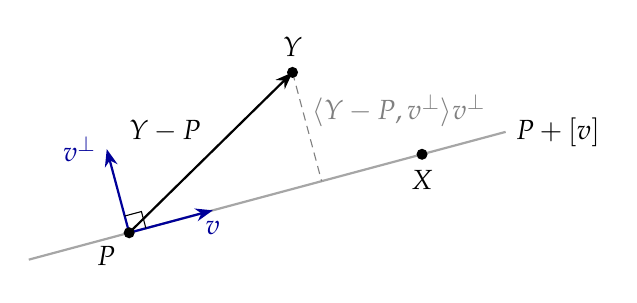
\begin{tikzpicture}[scale=1.1]
    \coordinate (P) at (0,0);
    \coordinate (F) at (15:2.3);
    \coordinate (Y) at ($(F)+(105:1.3)$);
    \coordinate (X) at (15:3.5);
    \draw[base, thick] (195:1.2) -- (15:4.5) node[right, black] {$P+[v]$};
    \draw[vec, mirrorc] (P) -- (15:1) node[below] {$v$};
    \draw[vec, mirrorc] (P) -- (105:1) node[left] {$v^\perp$};
    \draw (15:0.2) -- ($(15:0.2)+(105:0.2)$) -- (105:0.2);
    \draw[vec] (P) -- (Y) node[midway, above left] {$Y-P$};
    \draw[aux] (Y) -- (F);
    \node[gray, right] at ($(Y)!0.35!(F)$) {$\ip{Y-P}{v^\perp}v^\perp$};
    \node[pt, label=below left:{$P$}] at (P) {};
    \node[pt, label=below:{$X$}] at (X) {};
    \node[pt, label=above:{$Y$}] at (Y) {};
\end{tikzpicture}
\captionof{figure}{The line $P+[v]$ with a point $X$ on it and a point $Y$ off it.}\label{fig:normal}
\end{plate}

\begin{problem}[Parallel lines]\label{p:parallel}
Two distinct lines are \emph{parallel} if they have no point in common.\\
Let $\ell=P+[v]$ and $\ell'=P'+[v']$ be distinct lines.\\
Show that $\ell$ and $\ell'$ are parallel if and only if $v'$ is a multiple of $v$.
\end{problem}

\begin{solution}
\leavevmode
\begin{enumerate}[leftmargin=2.5em]
    \item[($\Leftarrow$)] Let $v'=cv$, where $c\neq0$ because $v'\neq0$.\\
    Suppose some point $X$ lies on both lines. Then Fact~\ref{f:anchor}(a) gives
    \[
    \ell=X+[v] \qquad\text{and}\qquad \ell'=X+[v']=X+[cv]=X+[v].
    \]
    So $\ell=\ell'$, which is excluded. Hence $\ell\cap\ell'=\varnothing$.
    \item[($\Rightarrow$)] We prove the contrapositive. Suppose $v'$ is not a multiple of $v$.\\
    Then $v$ and $v'$ are linearly independent.\\
    Indeed, if $av+bv'=0$ with $b\neq0$, then $v'=-(a/b)v$, which is excluded.\\
    So $b=0$, and then $av=0$ forces $a=0$.\\
    Hence $\{v,v'\}$ is a basis of $\R^2$, and $P'-P=tv-t'v'$ for some $t,t'\in\R$. The point
    \[
    X=P+tv=P'+t'v'
    \]
    lies on both lines, so they are not parallel. \qedhere
\end{enumerate}
\end{solution}

\begin{remark}
By Fact~\ref{f:anchor}(b) this does not depend on the choice of direction vectors.\\
Together with Problem~\ref{p:meet-once}, two distinct lines fall into exactly one of two cases (Figure~\ref{fig:parallel}).
\begin{itemize}[nosep]
    \item Parallel direction vectors and no common point.
    \item Non-parallel direction vectors and exactly one common point.
\end{itemize}
\end{remark}

\begin{plate}
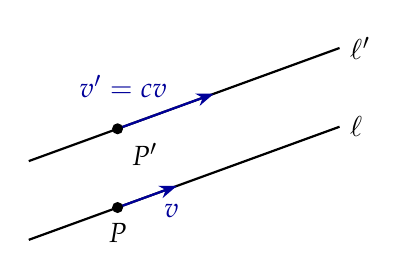
\begin{tikzpicture}
    \coordinate (P) at (0,0);
    \coordinate (P2) at (0,1);
    \draw[thick] (200:1.2) -- (20:3) node[right] {$\ell$};
    \draw[thick] ($(P2)+(200:1.2)$) -- ($(P2)+(20:3)$) node[right] {$\ell'$};
    \draw[vec, mirrorc] (P) -- (20:0.8);
    \node[mirrorc, below right] at (20:0.5) {$v$};
    \draw[vec, mirrorc] (P2) -- ($(P2)+(20:1.3)$);
    \node[mirrorc, above left] at ($(P2)+(20:0.8)$) {$v'=cv$};
    \node[pt, label=below:{$P$}] at (P) {};
    \node[pt, label=below right:{$P'$}] at (P2) {};
\end{tikzpicture}
\hspace{1.5cm}
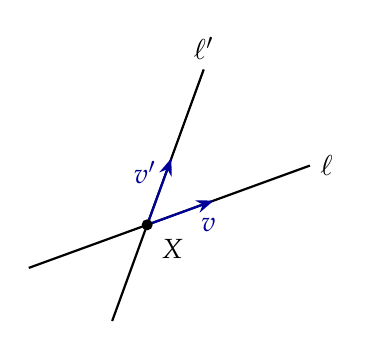
\begin{tikzpicture}
    \coordinate (X) at (0,0);
    \draw[thick] (200:1.6) -- (20:2.2) node[right] {$\ell$};
    \draw[thick] (250:1.3) -- (70:2.1) node[above] {$\ell'$};
    \draw[vec, mirrorc] (X) -- (20:0.9);
    \node[mirrorc, below right] at (20:0.6) {$v$};
    \draw[vec, mirrorc] (X) -- (70:0.9);
    \node[mirrorc, left] at (70:0.7) {$v'$};
    \node[pt, label=below right:{$X$}] at (X) {};
\end{tikzpicture}
\captionof{figure}{Left, two parallel lines. Right, two lines meeting at $X$.}\label{fig:parallel}
\end{plate}

\newpage
\section*{3. Reflections}

Below, $\boldsymbol{\ell}=P+[v]$ is a \textbf{line} with $\abs{v}=1$, which is possible by Fact~\ref{f:anchor}(a).\\
By Problem~\ref{p:normal}, $v^\perp$ is then a unit vector orthogonal to $v$.
\begin{description}
    \item[Reflection] The map $\Omega_\ell\colon\E\to\E$ with $\Omega_\ell(X)=X-2\ip{X-P}{v^\perp}v^\perp$.
\end{description}

\begin{note}
\leavevmode
\begin{enumerate}[label=\arabic*.]
    \item $\ip{X-P}{v^\perp}v^\perp$ is the part of $X-P$ perpendicular to $\ell$, and $\Omega_\ell$ reverses it (Figure~\ref{fig:reflection}).
    \item The formula uses a choice of $P$ and $v$, but the map depends only on $\ell$ (Fact~\ref{f:welldef}).
\end{enumerate}
\end{note}

\begin{fact}[The reflection depends only on the line]\label{f:welldef}
\leavevmode\\
Let $\ell=P+[v]=P'+[v']$ with $\abs{v}=\abs{v'}=1$.\\
Then for every point $X$
\[
\ip{X-P'}{v'^\perp}v'^\perp=\ip{X-P}{v^\perp}v^\perp.
\]
So the two formulas for $\Omega_\ell$ agree.
\end{fact}

\begin{proof}
\leavevmode\\
By Fact~\ref{f:anchor}(b), $v'$ is a multiple of $v$, and both have length $1$, so $v'=\pm v$.\\
Hence $v'^\perp=\pm v^\perp$, and the two signs cancel in $\ip{X-P'}{v'^\perp}v'^\perp$.\\
Also $P'\in\ell$, so $P'=P+sv$ for some $s$. Using $\ip{v}{v^\perp}=0$ we get
\[
\ip{X-P'}{v'^\perp}v'^\perp=\ip{X-P-sv}{v^\perp}v^\perp=\ip{X-P}{v^\perp}v^\perp. \qedhere
\]
\end{proof}

\begin{plate}
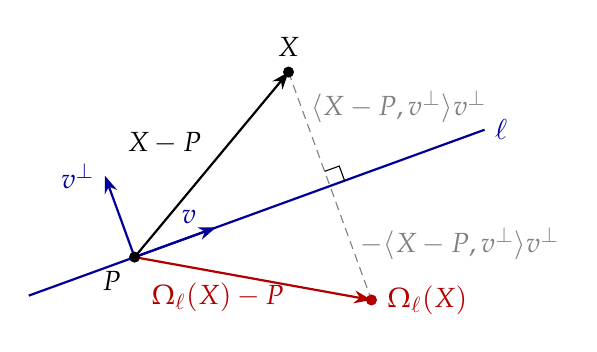
\begin{tikzpicture}[scale=1.1]
    \coordinate (P) at (0,0);
    \coordinate (F) at (20:2.4);
    \coordinate (X) at ($(F)+(110:1.4)$);
    \coordinate (Xr) at ($(F)+(-70:1.4)$);
    \draw[mirror] (200:1.3) -- (20:4.3) node[right] {$\ell$};
    \draw[aux] (X) -- (Xr);
    \draw ($(F)+(20:0.18)$) -- ($(F)+(20:0.18)+(110:0.18)$) -- ($(F)+(110:0.18)$);
    \draw[vec] (P) -- (X) node[midway, above left] {$X-P$};
    \draw[vec, imgc] (P) -- (Xr) node[pos=0.35, below] {$\Omega_\ell(X)-P$};
    \draw[vec, mirrorc] (P) -- (20:1);
    \node[mirrorc] at ($(20:0.75)+(110:0.22)$) {$v$};
    \draw[vec, mirrorc] (P) -- (110:1) node[left] {$v^\perp$};
    \node[gray, right] at ($(X)!0.3!(F)$) {$\ip{X-P}{v^\perp}v^\perp$};
    \node[gray, right] at ($(F)!0.5!(Xr)$) {$-\ip{X-P}{v^\perp}v^\perp$};
    \node[pt, label=above:{$X$}] at (X) {};
    \node[ipt, label={[imgc]right:{$\Omega_\ell(X)$}}] at (Xr) {};
    \node[pt, label=below left:{$P$}] at (P) {};
\end{tikzpicture}
\captionof{figure}{A point $X$ and its reflection $\Omega_\ell(X)$ in the line $\ell$.}\label{fig:reflection}
\end{plate}

\newpage
\begin{problem}[Reflections are bijections]\label{p:bijection}
Let $\ell=P+[v]$ be a line with $\abs{v}=1$, and let $\Omega_\ell$ be the reflection in $\ell$
\[
\Omega_\ell(X)=X-2\ip{X-P}{v^\perp}v^\perp.
\]
\begin{enumerate}
    \item Show that $\Omega_\ell\circ\Omega_\ell=\id$.
    \item Deduce that $\Omega_\ell$ is a bijection and $\Omega_\ell^{-1}=\Omega_\ell$.
\end{enumerate}
\end{problem}

\begin{solution}
\leavevmode\\
Write $n=v^\perp$, a unit vector.
\begin{enumerate}
    \item Fix a point $X$ and put $c=\ip{X-P}{n}$. Since $\ip{n}{n}=1$
    \[
    \ip{\Omega_\ell(X)-P}{n}=\ip{X-P-2cn}{n}=c-2c=-c.
    \]
    So the component along $n$ flips sign, as in Figure~\ref{fig:reflection}.\\
    Applying $\Omega_\ell$ again flips it back
    \[
    \Omega_\ell(\Omega_\ell(X))=\Omega_\ell(X)-2(-c)n=X-2cn+2cn=X.
    \]
    In Figure~\ref{fig:involution} (right), reflecting $X$ twice brings it back to $X$.
    \item We check the two halves of being a bijection.
    \begin{itemize}[nosep]
        \item \emph{Injective.} If $\Omega_\ell(X)=\Omega_\ell(Y)$, applying $\Omega_\ell$ and using (a) gives $X=Y$.
        \item \emph{Surjective.} Every point $Y$ equals $\Omega_\ell(\Omega_\ell(Y))$.
    \end{itemize}
    Since $\Omega_\ell\circ\Omega_\ell=\id$, the inverse of $\Omega_\ell$ is $\Omega_\ell$ itself.\\
    In Figure~\ref{fig:involution} (left), each point of $K$ is paired with exactly one point of $\Omega_\ell(K)$. \qedhere
\end{enumerate}
\end{solution}

\begin{plate}
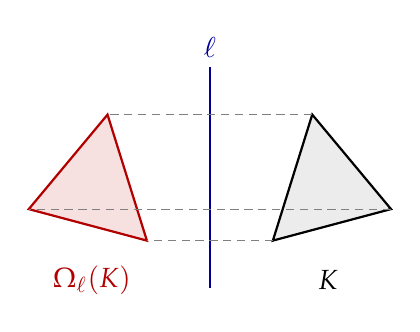
\begin{tikzpicture}
    \coordinate (A) at (0.8,0.2);
    \coordinate (B) at (2.3,0.6);
    \coordinate (C) at (1.3,1.8);
    \coordinate (Ar) at (-0.8,0.2);
    \coordinate (Br) at (-2.3,0.6);
    \coordinate (Cr) at (-1.3,1.8);
    \fill[gray!15] (A) -- (B) -- (C) -- cycle;
    \fill[imgc!12] (Ar) -- (Br) -- (Cr) -- cycle;
    \draw[thick] (A) -- (B) -- (C) -- cycle;
    \draw[thick, imgc] (Ar) -- (Br) -- (Cr) -- cycle;
    \draw[mirror] (0,-0.4) -- (0,2.4) node[above] {$\ell$};
    \draw[aux] (A) -- (Ar);
    \draw[aux] (B) -- (Br);
    \draw[aux] (C) -- (Cr);
    \node at (1.5,-0.3) {$K$};
    \node[imgc] at (-1.5,-0.3) {$\Omega_\ell(K)$};
\end{tikzpicture}
\hspace{1.5cm}
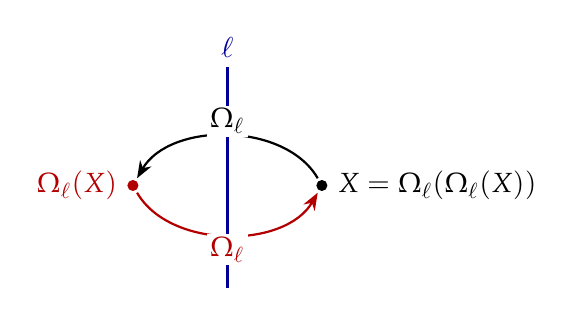
\begin{tikzpicture}
    \coordinate (X) at (1.2,0.9);
    \coordinate (Xr) at (-1.2,0.9);
    \draw[mirror] (0,-0.4) -- (0,2.4) node[above] {$\ell$};
    \draw[->, thick, shorten <=3pt, shorten >=3pt] (X) to[bend right=60] node[above, fill=white, inner sep=1pt] {$\Omega_\ell$} (Xr);
    \draw[->, thick, imgc, shorten <=3pt, shorten >=3pt] (Xr) to[bend right=60] node[below, fill=white, inner sep=1pt] {$\Omega_\ell$} (X);
    \node[pt, label=right:{$X=\Omega_\ell(\Omega_\ell(X))$}] at (X) {};
    \node[ipt, label={[imgc]left:{$\Omega_\ell(X)$}}] at (Xr) {};
\end{tikzpicture}
\captionof{figure}{Left, a triangle $K$ and its reflection. Right, a point $X$ reflected twice.}\label{fig:involution}
\end{plate}

\newpage
\begin{problem}[Reflections are isometries]\label{p:isometry}
Let $v$ be a unit vector.
\begin{enumerate}
    \item Show that every $w\in\R^2$ satisfies
    \[
    w-2\ip{w}{v^\perp}v^\perp=\ip{w}{v}v-\ip{w}{v^\perp}v^\perp.
    \]
    Deduce that $\abs{w-2\ip{w}{v^\perp}v^\perp}=\abs{w}$.
    \item Let $\ell=P+[v]$ and let $\Omega_\ell$ be the reflection in $\ell$.\\
    Show that $\Omega_\ell$ is an isometry, that is, for all points $X_1$ and $X_2$
    \[
    d(\Omega_\ell(X_1),\Omega_\ell(X_2))=d(X_1,X_2).
    \]
\end{enumerate}
\end{problem}

\begin{solution}
\leavevmode
\begin{enumerate}
    \item By Problem~\ref{p:normal}(a), $\{v,v^\perp\}$ is orthonormal, so Problem~\ref{p:orthonormal} gives
    \[
    w=\ip{w}{v}v+\ip{w}{v^\perp}v^\perp.
    \]
    Subtracting $2\ip{w}{v^\perp}v^\perp$ from both sides gives the identity.\\
    For the length, every $a,b\in\R$ satisfy
    \[
    \abs{av+bv^\perp}^2=a^2\ip{v}{v}+2ab\ip{v}{v^\perp}+b^2\ip{v^\perp}{v^\perp}=a^2+b^2.
    \]
    Take $a=\ip{w}{v}$ and $b=\pm\ip{w}{v^\perp}$.\\
    Then $w$ and $w-2\ip{w}{v^\perp}v^\perp$ both have squared length $\ip{w}{v}^2+\ip{w}{v^\perp}^2$.
    \item Subtracting the formulas for $\Omega_\ell(X_1)$ and $\Omega_\ell(X_2)$ gives
    \begin{align*}
    \Omega_\ell(X_1)-\Omega_\ell(X_2)
    &=(X_1-X_2)-2\bigl(\ip{X_1-P}{v^\perp}-\ip{X_2-P}{v^\perp}\bigr)v^\perp\\
    &=(X_1-X_2)-2\ip{X_1-X_2}{v^\perp}v^\perp.
    \end{align*}
    By (a) with $w=X_1-X_2$, this vector has length $\abs{X_1-X_2}=d(X_1,X_2)$.\\
    In Figure~\ref{fig:segment}, the segment and its image have the same length. \qedhere
\end{enumerate}
\end{solution}

\begin{plate}
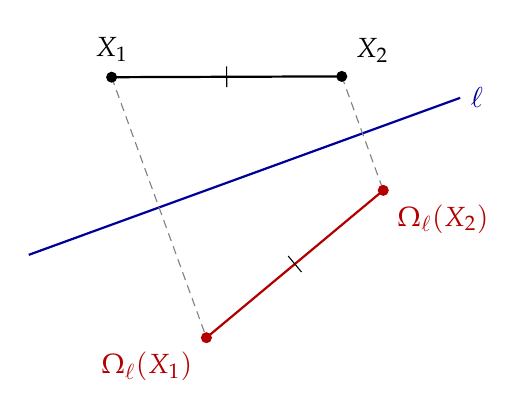
\begin{tikzpicture}[scale=1.1]
    \coordinate (A) at ($(20:0.6)+(110:1.6)$);
    \coordinate (B) at ($(20:3.1)+(110:0.7)$);
    \coordinate (Ar) at ($(20:0.6)+(-70:1.6)$);
    \coordinate (Br) at ($(20:3.1)+(-70:0.7)$);
    \draw[mirror] (200:1.0) -- (20:4.3) node[right] {$\ell$};
    \draw[aux] (A) -- (Ar);
    \draw[aux] (B) -- (Br);
    \draw[thick] (A) -- (B);
    \draw[thick, imgc] (Ar) -- (Br);
    \eqtick{A}{B}
    \eqtick{Ar}{Br}
    \node[pt, label=above:{$X_1$}] at (A) {};
    \node[pt, label=above right:{$X_2$}] at (B) {};
    \node[ipt, label={[imgc]below left:{$\Omega_\ell(X_1)$}}] at (Ar) {};
    \node[ipt, label={[imgc]below right:{$\Omega_\ell(X_2)$}}] at (Br) {};
\end{tikzpicture}
\captionof{figure}{A segment $X_1X_2$ and its reflection in $\ell$.}\label{fig:segment}
\end{plate}

\begin{problem}[The mirror is the fixed set]\label{p:fixed}
Let $\ell$ be a line and $\Omega_\ell$ the reflection in $\ell$.\\
Show that $\Omega_\ell(X)=X$ if and only if $X\in\ell$.\\
In other words, the points that $\Omega_\ell$ does not move are exactly the points of $\ell$.
\end{problem}

\begin{solution}
\leavevmode\\
Write $\ell=P+[v]$ with $\abs{v}=1$. Since $v^\perp\neq0$
\[
\Omega_\ell(X)=X
\iff 2\ip{X-P}{v^\perp}v^\perp=0
\iff \ip{X-P}{v^\perp}=0
\iff X\in\ell.
\]
The last step is Problem~\ref{p:normal}(b).
\end{solution}

\begin{problem}[The mirror as an equidistant set]\label{p:equidistant}
Let $\ell$ be a line and $Q$ a point not on $\ell$.\\
Show that a point $X$ lies on $\ell$ if and only if $d(X,Q)=d(X,\Omega_\ell(Q))$.
\end{problem}

\begin{solution}
\leavevmode\\
Write $\ell=P+[v]$ with $\abs{v}=1$ and put $n=v^\perp$.
\begin{enumerate}[leftmargin=2.5em]
    \item[($\Rightarrow$)] If $X\in\ell$, then $\Omega_\ell(X)=X$ by Problem~\ref{p:fixed}.\\
    Since $\Omega_\ell$ is an isometry (Problem~\ref{p:isometry}) we get
    \[
    d(X,\Omega_\ell(Q))=d(\Omega_\ell(X),\Omega_\ell(Q))=d(X,Q).
    \]
    \item[($\Leftarrow$)] Put $a=\ip{X-P}{n}$, $q=\ip{Q-P}{n}$ and $c=\ip{X-P}{v}-\ip{Q-P}{v}$.\\
    By Problem~\ref{p:orthonormal} applied to $\{v,n\}$, and since $\Omega_\ell(Q)-P=(Q-P)-2qn$
    \begin{align*}
    X-P &= \ip{X-P}{v}v+an\\
    Q-P &= \ip{Q-P}{v}v+qn\\
    \Omega_\ell(Q)-P &= \ip{Q-P}{v}v-qn.
    \end{align*}
    Subtracting gives
    \[
    X-Q=cv+(a-q)n \qquad\text{and}\qquad X-\Omega_\ell(Q)=cv+(a+q)n.
    \]
    As in Problem~\ref{p:isometry}(a), the squared distances are
    \[
    d(X,Q)^2=c^2+(a-q)^2 \qquad\text{and}\qquad d(X,\Omega_\ell(Q))^2=c^2+(a+q)^2.
    \]
    These are equal exactly when $(a+q)^2-(a-q)^2=4aq=0$.\\
    Since $Q\notin\ell$, Problem~\ref{p:normal}(b) gives $q\neq0$, so $a=0$ and $X\in\ell$.
\end{enumerate}
In Figure~\ref{fig:equidistant}, $X$ on $\ell$ is equally far from $Q$ and $\Omega_\ell(Q)$, while $Y$ off $\ell$ is not.
\end{solution}

\begin{remark}
The hypothesis $Q\notin\ell$ is needed only for ($\Leftarrow$).\\
If $Q\in\ell$, then $\Omega_\ell(Q)=Q$ and every point of the plane satisfies the equation.
\end{remark}

\begin{plate}
\begin{tikzpicture}
    \coordinate (Q) at (1.6,0.6);
    \coordinate (Qr) at (-1.6,0.6);
    \coordinate (X) at (0,2.2);
    \coordinate (Y) at (0.9,-1.3);
    \draw[mirror] (0,-2) -- (0,3) node[above] {$\ell$};
    \draw[aux] (Q) -- (Qr);
    \draw (X) -- (Q);
    \draw (X) -- (Qr);
    \eqtick{X}{Q}
    \eqtick{X}{Qr}
    \draw[gray, densely dotted, thick] (Y) -- (Q);
    \draw[gray, densely dotted, thick] (Y) -- (Qr);
    \node[pt, label=right:{$Q$}] at (Q) {};
    \node[ipt, label={[imgc]left:{$\Omega_\ell(Q)$}}] at (Qr) {};
    \node[pt, label=above right:{$X$}] at (X) {};
    \node[pt, label=below right:{$Y$}] at (Y) {};
\end{tikzpicture}
\captionof{figure}{A point $Q$, its reflection, and points $X$ on $\ell$ and $Y$ off $\ell$.}\label{fig:equidistant}
\end{plate}

\noindent Problem~\ref{p:equidistant} identifies the perpendicular bisector of a segment, which we use in Section~6.

\begin{corollary}[Perpendicular bisector]\label{c:bisector}
\leavevmode\\
Let $A\neq B$, and put $M=\tfrac12(A+B)$ and $u=(B-A)/\abs{B-A}$. Then
\[
\{X\in\E \mid d(X,A)=d(X,B)\}=M+[u^\perp].
\]
\end{corollary}

\begin{proof}
\leavevmode\\
Let $\ell=M+[u^\perp]$. Its unit direction is $u^\perp$, and $(u^\perp)^\perp=-u$, so
\[
\Omega_\ell(X)=X-2\ip{X-M}{-u}(-u)=X-2\ip{X-M}{u}u.
\]
Since $B-M=\tfrac12(B-A)=\tfrac12\abs{B-A}\,u$, we have $\ip{B-M}{u}=\tfrac12\abs{B-A}\neq0$.\\
Hence $B\notin\ell$ by Problem~\ref{p:normal}(b), and $\Omega_\ell(B)=B-\abs{B-A}\,u=A$.\\
Problem~\ref{p:equidistant} with $Q=B$ now shows that $X\in\ell$ exactly when $d(X,B)=d(X,A)$.\\
In Figure~\ref{fig:bisector}, $\Omega_\ell$ swaps $A$ and $B$, and $X$ on $\ell$ is equally far from both.
\end{proof}

\begin{plate}
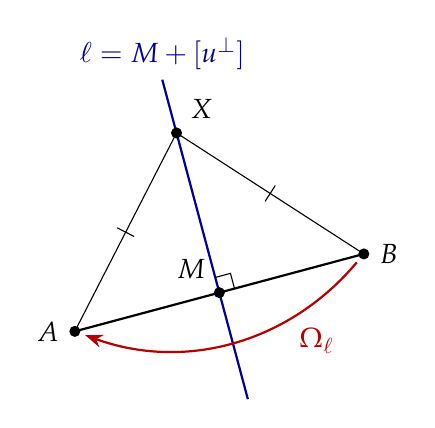
\begin{tikzpicture}
    \coordinate (M) at (0,0);
    \coordinate (A) at (195:1.9);
    \coordinate (B) at (15:1.9);
    \coordinate (X) at (105:2.1);
    \draw[mirror] (285:1.4) -- (105:2.8) node[above] {$\ell=M+[u^\perp]$};
    \draw[thick] (A) -- (B);
    \draw (X) -- (A);
    \draw (X) -- (B);
    \eqtick{X}{A}
    \eqtick{X}{B}
    \draw ($(M)+(15:0.2)$) -- ($(M)+(15:0.2)+(105:0.2)$) -- ($(M)+(105:0.2)$);
    \draw[->, thick, imgc, shorten <=4pt, shorten >=4pt] (B) to[bend left=35] node[pos=0.3, below right] {$\Omega_\ell$} (A);
    \node[pt, label=left:{$A$}] at (A) {};
    \node[pt, label=right:{$B$}] at (B) {};
    \node[pt, label=above left:{$M$}] at (M) {};
    \node[pt, label=above right:{$X$}] at (X) {};
\end{tikzpicture}
\captionof{figure}{A segment $AB$, its midpoint $M$ and its perpendicular bisector $\ell$.}\label{fig:bisector}
\end{plate}

\newpage
\section*{4. Rotations}

Below, $\boldsymbol{\theta}$ is a \textbf{real number} and $\boldsymbol{P}$ is a \textbf{point}.\\
When a matrix acts on a point, the point is written as a column.
\begin{description}
    \item[Rotation matrix] $\rot(\theta)=\bigl(\begin{smallmatrix}\cos\theta & -\sin\theta\\ \sin\theta & \cos\theta\end{smallmatrix}\bigr)$, also used as the map $X\mapsto\rot(\theta)X$.
    \item[Rotation about $\boldsymbol{P}$] $R_{P,\theta}(X)=P+\rot(\theta)(X-P)$, that is, $R_{P,\theta}=T_P\circ\rot(\theta)\circ T_{-P}$.
    \item[Angle] $\theta$ is an angle of the line $P+[(\cos\theta,\sin\theta)]$.
    \item[Perpendicular] Two lines are perpendicular if their direction vectors are orthogonal.
\end{description}

\begin{note}
\leavevmode
\begin{enumerate}[label=\arabic*.]
    \item $T_P$ is the translation by the vector $P$.\\
    So $R_{P,\theta}$ moves $P$ to the origin, turns by $\theta$, and moves back.
    \item Every unit vector is $(\cos\theta,\sin\theta)$ for some $\theta\in\R$, so every line has an angle.
\end{enumerate}
\end{note}

\begin{fact}[Reflections in lines through the origin]\label{f:matrix}
\leavevmode\\
Let $v=(\cos\theta,\sin\theta)$. The reflection in $[v]$ is the matrix
\[
S(2\theta)=\begin{pmatrix}\cos2\theta & \sin2\theta\\ \sin2\theta & -\cos2\theta\end{pmatrix}.
\]
Consequently, for $v_i=(\cos\theta_i,\sin\theta_i)$ with $i=1,2$
\[
\Omega_{[v_2]}\circ\Omega_{[v_1]}=\rot\bigl(2(\theta_2-\theta_1)\bigr).
\]
\end{fact}

\begin{proof}
\leavevmode\\
Put $n=v^\perp=(-\sin\theta,\cos\theta)$. Then $\Omega_{[v]}(x)=x-2\ip{x}{n}n=(I-2nn^{\top})x$, and
\[
I-2nn^{\top}=\begin{pmatrix}1-2\sin^2\theta & 2\sin\theta\cos\theta\\ 2\sin\theta\cos\theta & 1-2\cos^2\theta\end{pmatrix}=S(2\theta).
\]
For all $a$ and $b$, the addition formulas give
\[
S(a)S(b)=\begin{pmatrix}\cos a\cos b+\sin a\sin b & \cos a\sin b-\sin a\cos b\\ \sin a\cos b-\cos a\sin b & \sin a\sin b+\cos a\cos b\end{pmatrix}=\rot(a-b).
\]
Taking $a=2\theta_2$ and $b=2\theta_1$ gives the second claim.
\end{proof}

\begin{fact}[Moving the mirror off the origin]\label{f:conjugate}
\leavevmode\\
If $\ell=P+[v]$ with $\abs{v}=1$, then $\Omega_\ell=T_P\circ\Omega_{[v]}\circ T_{-P}$.
\end{fact}

\begin{proof}
\leavevmode\\
For every point $X$ we have $T_{-P}(X)=X-P$, so
\[
T_P\bigl(\Omega_{[v]}(X-P)\bigr)=(X-P)-2\ip{X-P}{v^\perp}v^\perp+P=\Omega_\ell(X). \qedhere
\]
\end{proof}

\begin{problem}[Adding angles]\label{p:addition}
Let $\theta,\theta'\in\R$.
\begin{enumerate}
    \item Show that $\rot(\theta)\rot(\theta')=\rot(\theta+\theta')$.
    \item Deduce that $\rot(\theta)$ is invertible with inverse $\rot(-\theta)$.
    \item Deduce that $\rot(\theta)\rot(\theta')=\rot(\theta')\rot(\theta)$.
\end{enumerate}
\end{problem}

\begin{solution}
\leavevmode
\begin{enumerate}
    \item Multiplying out gives
    \[
    \rot(\theta)\rot(\theta')=\begin{pmatrix}\cos\theta\cos\theta'-\sin\theta\sin\theta' & -(\sin\theta\cos\theta'+\cos\theta\sin\theta')\\ \sin\theta\cos\theta'+\cos\theta\sin\theta' & \cos\theta\cos\theta'-\sin\theta\sin\theta'\end{pmatrix}.
    \]
    The addition formulas
    \begin{align*}
    \cos(\alpha+\beta) &= \cos\alpha\cos\beta-\sin\alpha\sin\beta\\
    \sin(\alpha+\beta) &= \sin\alpha\cos\beta+\cos\alpha\sin\beta
    \end{align*}
    turn the entries into those of $\rot(\theta+\theta')$
    \[
    \rot(\theta)\rot(\theta')=\begin{pmatrix}\cos(\theta+\theta') & -\sin(\theta+\theta')\\ \sin(\theta+\theta') & \cos(\theta+\theta')\end{pmatrix}=\rot(\theta+\theta').
    \]
    In Figure~\ref{fig:addition}, turning $e_1$ by $\theta'$ and then by $\theta$ lands at angle $\theta+\theta'$.
    \item By (a) with $\theta'=-\theta$, and since $\rot(0)=I$
    \[
    \rot(\theta)\rot(-\theta)=\rot(0)=I=\rot(-\theta)\rot(\theta).
    \]
    So $\rot(\theta)$ is invertible with inverse $\rot(-\theta)$.
    \item By (a), both products equal $\rot(\theta+\theta')=\rot(\theta'+\theta)$. \qedhere
\end{enumerate}
\end{solution}

\begin{plate}
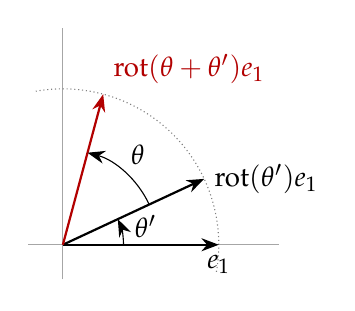
\begin{tikzpicture}[scale=1.1]
    \draw[base] (-0.4,0) -- (2.5,0);
    \draw[base] (0,-0.4) -- (0,2.5);
    \draw[gray, densely dotted] (-10:1.8) arc (-10:100:1.8);
    \draw[vec] (0,0) -- (0:1.8) node[below] {$e_1$};
    \draw[vec] (0,0) -- (25:1.8) node[right] {$\rot(\theta')e_1$};
    \draw[vec, imgc] (0,0) -- (75:1.8) node[above right] {$\rot(\theta+\theta')e_1$};
    \draw[->] (0:0.7) arc (0:25:0.7);
    \node at (12.5:0.98) {$\theta'$};
    \draw[->] (25:1.1) arc (25:75:1.1);
    \node at (50:1.35) {$\theta$};
\end{tikzpicture}
\captionof{figure}{The vector $e_1$ turned by $\theta'$ and then by $\theta$.}\label{fig:addition}
\end{plate}

\begin{problem}[Two mirrors through a point]\label{p:two-mirrors}
Let $P$ be a point.\\
For $i=1,2$ let $\theta_i\in\R$, $v_i=(\cos\theta_i,\sin\theta_i)$ and $\ell_i=P+[v_i]$. Show that
\[
\Omega_{\ell_2}\circ\Omega_{\ell_1}=T_P\circ\rot\bigl(2(\theta_2-\theta_1)\bigr)\circ T_{-P}=R_{P,2(\theta_2-\theta_1)}.
\]
In words, reflecting in two lines through $P$ is the same as rotating about $P$ by twice the angle from the first line to the second.
\end{problem}

\begin{solution}
\leavevmode\\
By Fact~\ref{f:conjugate}, $\Omega_{\ell_i}=T_P\circ\Omega_{[v_i]}\circ T_{-P}$ for $i=1,2$. Since $T_{-P}\circ T_P=\id$
\begin{align*}
\Omega_{\ell_2}\circ\Omega_{\ell_1}
&=T_P\circ\Omega_{[v_2]}\circ(T_{-P}\circ T_P)\circ\Omega_{[v_1]}\circ T_{-P}\\
&=T_P\circ\bigl(\Omega_{[v_2]}\circ\Omega_{[v_1]}\bigr)\circ T_{-P}\\
&=T_P\circ\rot\bigl(2(\theta_2-\theta_1)\bigr)\circ T_{-P}.
\end{align*}
The last step is Fact~\ref{f:matrix}.\\
In Figure~\ref{fig:two-mirrors}, the mirrors meet at angle $\alpha=\theta_2-\theta_1$ and $X$ turns about $P$ by $2\alpha$.
\end{solution}

\begin{plate}
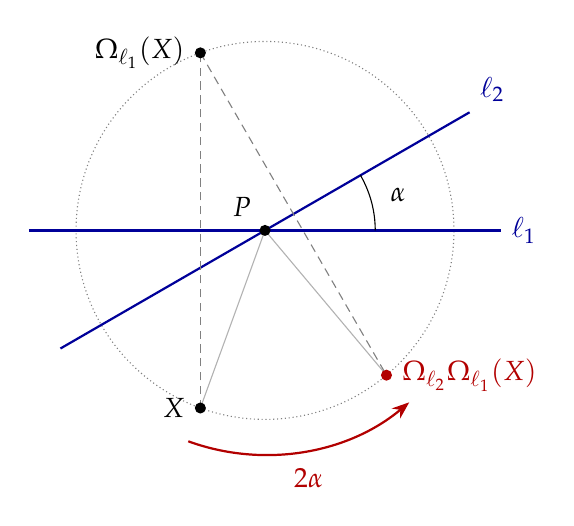
\begin{tikzpicture}
    \coordinate (P) at (0,0);
    \coordinate (X) at (-110:2.4);
    \coordinate (X1) at (110:2.4);
    \coordinate (X2) at (-50:2.4);
    \draw[gray, densely dotted] (P) circle (2.4);
    \draw[gray!60] (P) -- (X);
    \draw[gray!60] (P) -- (X2);
    \draw[mirror] (180:3.0) -- (0:3.0) node[right] {$\ell_1$};
    \draw[mirror] (210:3.0) -- (30:3.0) node[above right] {$\ell_2$};
    \draw[aux] (X) -- (X1);
    \draw[aux] (X1) -- (X2);
    \draw (0:1.4) arc (0:30:1.4);
    \node at (15:1.75) {$\alpha$};
    \draw[->, imgc, thick] (-110:2.85) arc (-110:-50:2.85);
    \node[imgc] at (-80:3.2) {$2\alpha$};
    \node[pt, label=left:{$X$}] at (X) {};
    \node[pt, label=left:{$\Omega_{\ell_1}(X)$}] at (X1) {};
    \node[ipt, label={[imgc]right:{$\Omega_{\ell_2}\Omega_{\ell_1}(X)$}}] at (X2) {};
    \node[pt, label=above left:{$P$}] at (P) {};
\end{tikzpicture}
\captionof{figure}{Two mirrors through $P$ at angle $\alpha$, and a point $X$ reflected in both.}\label{fig:two-mirrors}
\end{plate}

\begin{remark}
Three consequences are used below.
\begin{enumerate}[label=(\roman*)]
    \item \emph{Only the angle matters.}\\
    The composition depends on the two lines only through $P$ and $\theta_2-\theta_1$.\\
    So pairs of lines through $P$ with the same angle difference give the same rotation.
    \item \emph{Perpendicular mirrors give a half-turn.}\\
    If $\theta_2-\theta_1=\pi/2+k\pi$ with $k\in\mathbb{Z}$, then $\rot\bigl(2(\theta_2-\theta_1)\bigr)=-I$.\\
    So $\Omega_{\ell_2}\circ\Omega_{\ell_1}=R_{P,\pi}$, the map $X\mapsto2P-X$.
    \item \emph{Equal lines.}\\
    The lines $\ell_1$ and $\ell_2$ coincide exactly when $\theta_2-\theta_1$ is a multiple of $\pi$.\\
    Equal lines have $v_2=\pm v_1$ by Fact~\ref{f:anchor}(b), and $v_2=\pm v_1$ gives equal lines by Fact~\ref{f:anchor}(a).
\end{enumerate}
\end{remark}

\begin{problem}[Three mirrors through a point]\label{p:three-concurrent}
Let $P$ be a point, let $v_1,v_2,v_3$ be unit vectors and let $\ell_i=P+[v_i]$.\\
Show that there is a unit vector $v_4$ such that the line $\ell_4=P+[v_4]$ satisfies
\[
\Omega_{\ell_3}\circ\Omega_{\ell_2}\circ\Omega_{\ell_1}=\Omega_{\ell_4}.
\]
\end{problem}

\begin{solution}
\leavevmode\\
The idea is to trade the pair $\ell_2,\ell_3$ for a pair $\ell_1,\ell_4$ with the same angle difference.\\
Write $v_i=(\cos\theta_i,\sin\theta_i)$ for $i=1,2,3$, and set
\[
\theta_4=\theta_1-\theta_2+\theta_3, \qquad v_4=(\cos\theta_4,\sin\theta_4), \qquad \ell_4=P+[v_4].
\]
Since $\theta_4-\theta_1=\theta_3-\theta_2$, Problem~\ref{p:two-mirrors} gives
\[
\Omega_{\ell_4}\circ\Omega_{\ell_1}=R_{P,2(\theta_4-\theta_1)}=R_{P,2(\theta_3-\theta_2)}=\Omega_{\ell_3}\circ\Omega_{\ell_2}.
\]
Composing on the right with $\Omega_{\ell_1}$ and using $\Omega_{\ell_1}\circ\Omega_{\ell_1}=\id$ (Problem~\ref{p:bijection}) gives
\[
\Omega_{\ell_4}=\Omega_{\ell_4}\circ\Omega_{\ell_1}\circ\Omega_{\ell_1}=\Omega_{\ell_3}\circ\Omega_{\ell_2}\circ\Omega_{\ell_1}.
\]
In Figure~\ref{fig:three-mirrors}, $\ell_4$ is $\ell_1$ turned about $P$ by the angle $\beta=\theta_3-\theta_2$ from $\ell_2$ to $\ell_3$.
\end{solution}

\begin{plate}
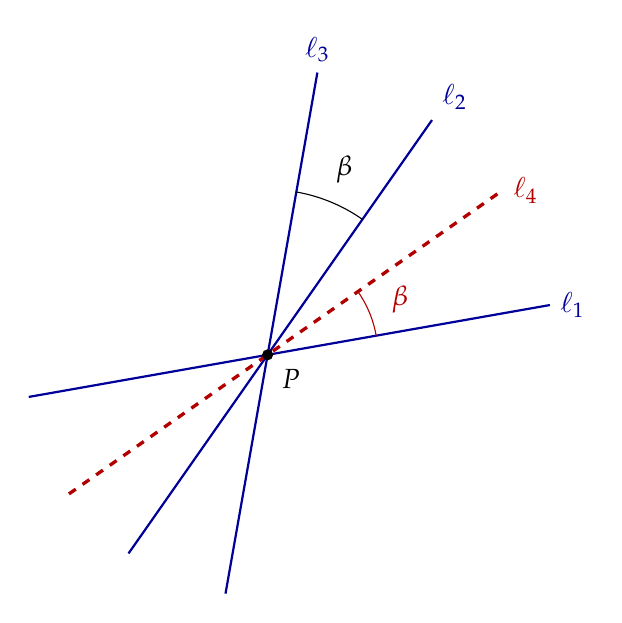
\begin{tikzpicture}[scale=1.4]
    \draw[mirror] (190:2.2) -- (10:2.6) node[right] {$\ell_1$};
    \draw[mirror] (235:2.2) -- (55:2.6) node[above right] {$\ell_2$};
    \draw[mirror] (260:2.2) -- (80:2.6) node[above] {$\ell_3$};
    \draw[very thick, imgc, dashed] (215:2.2) -- (35:2.6) node[right] {$\ell_4$};
    \draw (55:1.5) arc (55:80:1.5);
    \node at (67.5:1.82) {$\beta$};
    \draw[imgc] (10:1.0) arc (10:35:1.0);
    \node[imgc] at (22.5:1.3) {$\beta$};
    \node[pt, label=below right:{$P$}] at (0,0) {};
\end{tikzpicture}
\captionof{figure}{Three mirrors $\ell_1,\ell_2,\ell_3$ through $P$ and the fourth mirror $\ell_4$.}\label{fig:three-mirrors}
\end{plate}

\newpage
\section*{5. Glide Reflections}

Below, $\boldsymbol{\ell}=P+[v]$ is a \textbf{line} with $\abs{v}=1$ and $n=v^\perp$, and $\boldsymbol{w}$ and $\boldsymbol{y}$ are \textbf{vectors}.
\begin{description}
    \item[Parallel to $\boldsymbol{\ell}$] $w$ is a multiple of $v$.
    \item[Glide reflection] The map $T_w\circ\Omega_\ell$ with $w\neq0$ parallel to $\ell$.
    \item[Axis] The line $\ell$ of a glide reflection $T_w\circ\Omega_\ell$.
    \item[Vector reflection] $S_\ell(y)=y-2\ip{y}{n}n$, which flips the component of $y$ along $n$.
\end{description}

\begin{note}
\leavevmode
\begin{enumerate}[label=\arabic*.]
    \item Unlike parallel vectors in 1.1, a vector parallel to $\ell$ may be $0$.
    \item As in Fact~\ref{f:welldef}, $S_\ell$ does not depend on the sign of $n$.
\end{enumerate}
\end{note}

\begin{fact}[Reflections and translations]\label{f:slide}
\leavevmode\\
For every vector $y$ we have $\Omega_\ell\circ T_y=T_{S_\ell(y)}\circ\Omega_\ell$.
\end{fact}

\begin{proof}
\leavevmode\\
For every point $X$
\[
\Omega_\ell(X+y)=X+y-2\ip{X-P}{n}n-2\ip{y}{n}n=\Omega_\ell(X)+S_\ell(y).
\]
In words, $\Omega_\ell$ turns a translation by $y$ into a translation by $S_\ell(y)$.
\end{proof}

\begin{fact}[Parallel mirrors]\label{f:parallel-mirrors}
\leavevmode\\
Let $\ell=A+[v]$ and $m=B+[v]$ with $\abs{v}=1$, and put $n=v^\perp$. Then
\[
\Omega_m\circ\Omega_\ell=T_{2\ip{B-A}{n}n}.
\]
The vector $\ip{B-A}{n}n$ is $0$ exactly when $\ell=m$.
\end{fact}

\begin{proof}
\leavevmode\\
Fix a point $X$ and put $c=\ip{X-A}{n}$.\\
As in Problem~\ref{p:bijection}(a), $\ip{\Omega_\ell(X)-A}{n}=-c$.\\
Hence $\ip{\Omega_\ell(X)-B}{n}=-c-\ip{B-A}{n}$, and therefore
\begin{align*}
\Omega_m(\Omega_\ell(X)) &= \Omega_\ell(X)+2\bigl(c+\ip{B-A}{n}\bigr)n\\
&= X-2cn+2cn+2\ip{B-A}{n}n\\
&= X+2\ip{B-A}{n}n.
\end{align*}
By Problem~\ref{p:normal}(b), $\ip{B-A}{n}=0$ exactly when $B\in\ell$.\\
By Fact~\ref{f:anchor}(a) this happens exactly when $m=\ell$.
\end{proof}

\begin{problem}[Sliding along the mirror]\label{p:commute}
Let $\ell=P+[v]$ be a line with $\abs{v}=1$, and let $w$ be a vector parallel to $\ell$.\\
Show that $T_w\circ\Omega_\ell=\Omega_\ell\circ T_w$.
\end{problem}

\begin{solution}
\leavevmode\\
Write $w=cv$. Then $\ip{w}{v^\perp}=c\ip{v}{v^\perp}=0$, so $S_\ell(w)=w$.\\
Fact~\ref{f:slide} now gives $\Omega_\ell\circ T_w=T_{S_\ell(w)}\circ\Omega_\ell=T_w\circ\Omega_\ell$.\\
In Figure~\ref{fig:commute}, both paths from $X$ end at the same point.
\end{solution}

\begin{remark}
So a glide reflection can be written in either order.\\
Problem~\ref{p:commutator} shows that the condition on $w$ cannot be dropped.
\end{remark}

\begin{plate}
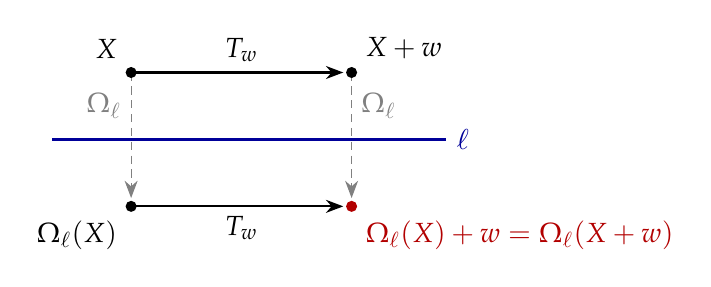
\begin{tikzpicture}
    \coordinate (X) at (0,0.85);
    \coordinate (Xr) at (0,-0.85);
    \coordinate (Xw) at (2.8,0.85);
    \coordinate (Xrw) at (2.8,-0.85);
    \draw[mirror] (-1,0) -- (4,0) node[right] {$\ell$};
    \draw[->, aux, shorten >=3pt] (X) -- (Xr) node[pos=0.25, left] {$\Omega_\ell$};
    \draw[->, thick, shorten >=3pt] (Xr) -- (Xrw) node[midway, below] {$T_w$};
    \draw[->, thick, shorten >=3pt] (X) -- (Xw) node[midway, above] {$T_w$};
    \draw[->, aux, shorten >=3pt] (Xw) -- (Xrw) node[pos=0.25, right] {$\Omega_\ell$};
    \node[pt, label=above left:{$X$}] at (X) {};
    \node[pt, label=below left:{$\Omega_\ell(X)$}] at (Xr) {};
    \node[pt, label=above right:{$X+w$}] at (Xw) {};
    \node[ipt, label={[imgc]below right:{$\Omega_\ell(X)+w=\Omega_\ell(X+w)$}}] at (Xrw) {};
\end{tikzpicture}
\captionof{figure}{A point $X$ reflected in $\ell$ and translated by $w$, in both orders.}\label{fig:commute}
\end{plate}

\begin{problem}[The square of a glide reflection]\label{p:glide-square}
Let $\gamma=T_w\circ\Omega_\ell$ be a glide reflection, so $w\neq0$ is parallel to $\ell$.
\begin{enumerate}
    \item Show that $\gamma\circ\gamma=T_{2w}$.
    \item Deduce that $\gamma$ has no fixed point.
\end{enumerate}
\end{problem}

\begin{solution}
\leavevmode
\begin{enumerate}
    \item The middle factors commute by Problem~\ref{p:commute}, and $\Omega_\ell\circ\Omega_\ell=\id$ by Problem~\ref{p:bijection}. So
    \[
    \gamma\circ\gamma=T_w\circ\Omega_\ell\circ T_w\circ\Omega_\ell=T_w\circ T_w\circ\Omega_\ell\circ\Omega_\ell=T_{2w}.
    \]
    \item Suppose $\gamma(X)=X$. Then also $\gamma(\gamma(X))=X$.\\
    But by (a), $\gamma(\gamma(X))=X+2w\neq X$, since $w\neq0$.\\
    In Figure~\ref{fig:footprints}, no footprint stays put, and two steps make $T_{2w}$. \qedhere
\end{enumerate}
\end{solution}

\begin{plate}
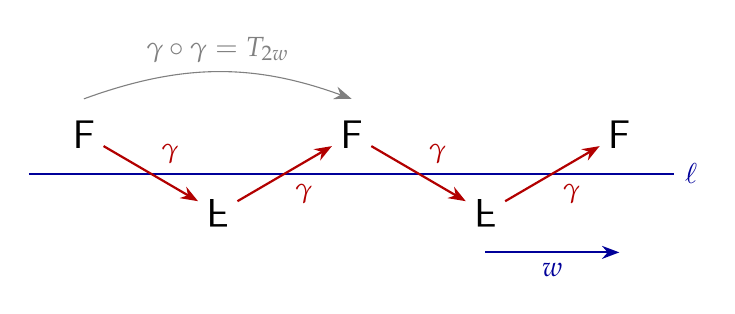
\begin{tikzpicture}
    \draw[mirror] (-0.7,0) -- (7.5,0) node[right] {$\ell$};
    \foreach \k in {0,2,4} {
        \node at (1.7*\k,0.5) {\Large\textsf{F}};
    }
    \foreach \k in {1,3} {
        \node at (1.7*\k,-0.5) {\scalebox{1}[-1]{\Large\textsf{F}}};
    }
    \draw[->, imgc, thick] (0.25,0.35) -- (1.45,-0.35) node[midway, above right] {$\gamma$};
    \draw[->, imgc, thick] (1.95,-0.35) -- (3.15,0.35) node[midway, below right] {$\gamma$};
    \draw[->, imgc, thick] (3.65,0.35) -- (4.85,-0.35) node[midway, above right] {$\gamma$};
    \draw[->, imgc, thick] (5.35,-0.35) -- (6.55,0.35) node[midway, below right] {$\gamma$};
    \draw[->, gray] (0,0.95) to[bend left=20] node[above] {$\gamma\circ\gamma=T_{2w}$} (3.4,0.95);
    \draw[vec, mirrorc] (5.1,-1.0) -- (6.8,-1.0) node[midway, below] {$w$};
\end{tikzpicture}
\captionof{figure}{Footprints moved along the axis $\ell$ by a glide reflection $\gamma$.}\label{fig:footprints}
\end{plate}

\begin{problem}[A commutator]\label{p:commutator}
Let $\ell=P+[u]$ be a line with $\abs{u}=1$, put $n=u^\perp$, and let $v$ be any vector.\\
The \emph{commutator} of $T_v$ and $\Omega_\ell$ is
\[
[T_v,\Omega_\ell]=T_v\circ\Omega_\ell\circ T_{-v}\circ\Omega_\ell.
\]
\begin{enumerate}
    \item Show that $[T_v,\Omega_\ell]=T_{2\ip{v}{n}n}$.\\
    This is the translation by twice the component of $v$ perpendicular to $\ell$.
    \item Show that $[T_v,\Omega_\ell]=\id$ if and only if $v$ is parallel to $\ell$.\\
    Show that this happens exactly when $T_v$ and $\Omega_\ell$ commute.
\end{enumerate}
\end{problem}

\begin{solution}
\leavevmode
\begin{enumerate}
    \item Fact~\ref{f:slide} with $y=-v$ gives
    \[
    \Omega_\ell\circ T_{-v}=T_{S_\ell(-v)}\circ\Omega_\ell=T_{-S_\ell(v)}\circ\Omega_\ell.
    \]
    With $\Omega_\ell\circ\Omega_\ell=\id$ (Problem~\ref{p:bijection}) this gives
    \[
    [T_v,\Omega_\ell]=T_v\circ T_{-S_\ell(v)}\circ\Omega_\ell\circ\Omega_\ell=T_{v-S_\ell(v)}=T_{2\ip{v}{n}n}.
    \]
    In Figure~\ref{fig:commutator}, the part of $v$ along $\ell$ cancels and the part along $n$ doubles.
    \item A translation $T_y$ is the identity exactly when $y=0$.\\
    So $[T_v,\Omega_\ell]=\id$ exactly when $\ip{v}{n}=0$.\\
    By Problem~\ref{p:orthonormal} applied to $\{u,n\}$ we have $v=\ip{v}{u}u+\ip{v}{n}n$.\\
    So $\ip{v}{n}=0$ exactly when $v$ is a multiple of $u$, that is, parallel to $\ell$.\\
    Finally, since $T_{-v}=T_v^{-1}$ and $\Omega_\ell=\Omega_\ell^{-1}$
    \[
    [T_v,\Omega_\ell]=\id
    \iff T_v\circ\Omega_\ell=(T_{-v}\circ\Omega_\ell)^{-1}=\Omega_\ell\circ T_v. \qedhere
    \]
\end{enumerate}
\end{solution}

\begin{plate}
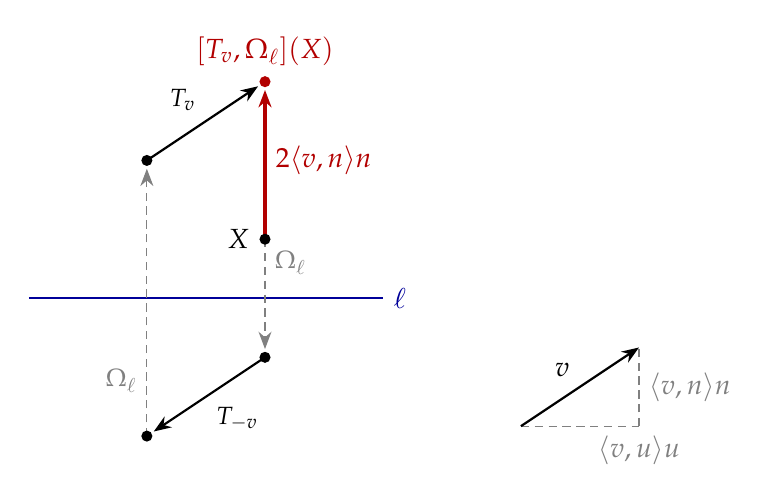
\begin{tikzpicture}[scale=1.25]
    \coordinate (X) at (0,0.6);
    \coordinate (X1) at (0,-0.6);
    \coordinate (X2) at (-1.2,-1.4);
    \coordinate (X3) at (-1.2,1.4);
    \coordinate (X4) at (0,2.2);
    \draw[mirror] (-2.4,0) -- (1.2,0) node[right] {$\ell$};
    \draw[->, aux, shorten >=3pt] (X) -- (X1) node[pos=0.2, right] {\small $\Omega_\ell$};
    \draw[->, thick, shorten >=3pt] (X1) -- (X2) node[midway, below right] {\small $T_{-v}$};
    \draw[->, aux, shorten >=3pt] (X2) -- (X3) node[pos=0.2, left] {\small $\Omega_\ell$};
    \draw[->, thick, shorten >=3pt] (X3) -- (X4) node[midway, above left] {\small $T_v$};
    \draw[->, very thick, imgc, shorten >=3pt] (X) -- (X4) node[midway, right] {$2\ip{v}{n}n$};
    \node[pt, label=left:{$X$}] at (X) {};
    \node[pt] at (X1) {};
    \node[pt] at (X2) {};
    \node[pt] at (X3) {};
    \node[ipt, label={[imgc]above:{$[T_v,\Omega_\ell](X)$}}] at (X4) {};
    \begin{scope}[shift={(2.6,-1.3)}]
        \draw[aux] (0,0) -- (1.2,0) node[below] {$\ip{v}{u}u$};
        \draw[aux] (1.2,0) -- (1.2,0.8) node[midway, right] {$\ip{v}{n}n$};
        \draw[vec] (0,0) -- (1.2,0.8) node[midway, above left] {$v$};
    \end{scope}
\end{tikzpicture}
\captionof{figure}{The four steps of $[T_v,\Omega_\ell]$ applied to $X$, and the two parts of $v$.}\label{fig:commutator}
\end{plate}

\begin{problem}[Three mirrors in general position]\label{p:general}
The following terms are for three lines, of which some may coincide.
\begin{description}
    \item[Concurrent] Some point lies on all three lines.
    \item[Share a direction] Their direction vectors are pairwise parallel.
\end{description}
A glide reflection is a map $T_w\circ\Omega_k$ with $k$ a line and $w\neq0$ parallel to $k$.\\
Let $\ell_1,\ell_2,\ell_3$ be lines that are neither concurrent nor share a direction.\\
Show that $\Omega_{\ell_3}\circ\Omega_{\ell_2}\circ\Omega_{\ell_1}$ is a glide reflection.
\end{problem}

\begin{solution}
\leavevmode\\
Write $T=\Omega_{\ell_3}\circ\Omega_{\ell_2}\circ\Omega_{\ell_1}$.\\
The idea is to turn the mirrors without changing $T$ until two are parallel.\\
Recall that lines with non-parallel directions meet exactly once (Problems~\ref{p:meet-once} and~\ref{p:parallel}).

\medskip\noindent
\textbf{Case 1.} The direction vectors of $\ell_1$ and $\ell_2$ are not parallel.\\
Then $\ell_1$ and $\ell_2$ meet at a single point $A$, and $A\notin\ell_3$ because the lines are not concurrent.\\
By Fact~\ref{f:anchor} we can write
\[
\ell_1=A+[(\cos\alpha_1,\sin\alpha_1)], \qquad
\ell_2=A+[(\cos\alpha_2,\sin\alpha_2)], \qquad
\ell_3=C+[(\cos\beta,\sin\beta)]
\]
for some point $C$ and angles $\alpha_1$, $\alpha_2$ and $\beta$.

\smallskip\noindent
\textit{Step 1. Turn the pair $\ell_1,\ell_2$ about $A$} (Figure~\ref{fig:general}(b)).\\
Let $\ell_2'$ be the line through $A$ with angle $\beta+\pi/2$. It is perpendicular to $\ell_3$.\\
Let $\ell_1'$ be the line through $A$ with angle $\alpha_1'=\alpha_1+(\beta+\pi/2)-\alpha_2$.\\
The angle from $\ell_1'$ to $\ell_2'$ is again $\alpha_2-\alpha_1$, so Problem~\ref{p:two-mirrors} gives
\[
\Omega_{\ell_2}\circ\Omega_{\ell_1}=R_{A,2(\alpha_2-\alpha_1)}=\Omega_{\ell_2'}\circ\Omega_{\ell_1'}.
\]
As $\ell_1\neq\ell_2$ and the angle differences agree, $\ell_1'\neq\ell_2'$ by Remark~(iii) after Problem~\ref{p:two-mirrors}.\\
Hence $T=\Omega_{\ell_3}\circ\Omega_{\ell_2'}\circ\Omega_{\ell_1'}$.

\smallskip\noindent
\textit{Step 2. Turn the pair $\ell_2',\ell_3$ about $B$} (Figure~\ref{fig:general}(c)).\\
The lines $\ell_2'$ and $\ell_3$ have orthogonal direction vectors, so they meet at a single point $B$.\\
Since $A\in\ell_2'$ but $A\notin\ell_3$, we have $B\neq A$.\\
Both lines pass through $B$, so Remark~(ii) after Problem~\ref{p:two-mirrors} gives $\Omega_{\ell_3}\circ\Omega_{\ell_2'}=R_{B,\pi}$.\\
Let $u=(\cos\alpha_1',\sin\alpha_1')$, a unit direction of $\ell_1'$, and put $m=B+[u]$ and $k=B+[u^\perp]$.\\
These are perpendicular lines through $B$, so again $R_{B,\pi}=\Omega_k\circ\Omega_m$. Hence
\[
T=\Omega_k\circ\Omega_m\circ\Omega_{\ell_1'}.
\]

\newpage\noindent
\textit{Step 3. The parallel pair $\ell_1',m$ gives a translation.}\\
The lines $\ell_1'=A+[u]$ and $m=B+[u]$ share the direction $u$, so Fact~\ref{f:parallel-mirrors} gives
\[
\Omega_m\circ\Omega_{\ell_1'}=T_w \qquad\text{with}\qquad w=2\ip{B-A}{u^\perp}u^\perp.
\]
Suppose $w=0$. Then Fact~\ref{f:parallel-mirrors} gives $m=\ell_1'$, so $B\in\ell_1'$.\\
But $B\in\ell_2'$, and the distinct lines $\ell_1'$ and $\ell_2'$ meet only at $A$ (Problem~\ref{p:meet-once}).\\
So $B=A$, which is false. Hence $w\neq0$.

\smallskip\noindent
\textit{Step 4. Conclusion} (Figure~\ref{fig:general}(d)).\\
Now $T=\Omega_k\circ T_w$, where $w\neq0$ is a multiple of $u^\perp$, the direction of $k$.\\
By Problem~\ref{p:commute}, $T=T_w\circ\Omega_k$, a glide reflection with axis $k$.\\
In Figure~\ref{fig:general}(d), the three reflections (dotted) and the glide send $X$ to the same point.

\medskip\noindent
\textbf{Case 2.} The direction vectors of $\ell_1$ and $\ell_2$ are parallel.\\
Then those of $\ell_2$ and $\ell_3$ are not, since otherwise all three lines would share a direction.\\
By Problem~\ref{p:bijection}, $T^{-1}=\Omega_{\ell_1}\circ\Omega_{\ell_2}\circ\Omega_{\ell_3}$.\\
This is the same kind of product for the lines $\ell_3,\ell_2,\ell_1$ taken in this order.\\
These lines satisfy the hypotheses, and the first two have non-parallel direction vectors.\\
By Case~1, $T^{-1}=T_w\circ\Omega_k$ for some line $k$ and some $w\neq0$ parallel to $k$.\\
Then Problem~\ref{p:commute} gives
\[
T=\Omega_k^{-1}\circ T_w^{-1}=\Omega_k\circ T_{-w}=T_{-w}\circ\Omega_k.
\]
This is a glide reflection, since $-w\neq0$ is parallel to $k$.
\end{solution}

\begin{plate}
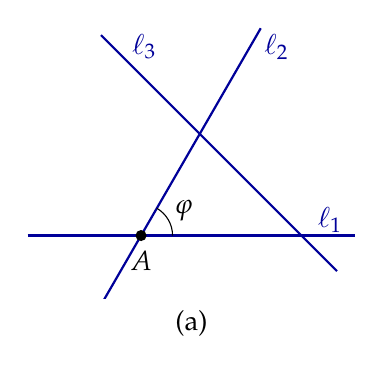
\begin{tikzpicture}[scale=0.8]
    \begin{scope}
        \clip (-1.8,-1.0) rectangle (3.4,3.3);
        \coordinate (A) at (0,0);
        \coordinate (B) at (45:1.8);
        \draw[mirror] (180:1.8) -- (0:3.4);
        \draw[mirror] (240:1.7) -- (60:3.8);
        \draw[mirror] ($(B)+(135:2.7)$) -- ($(B)+(-45:2.6)$);
        \node[mirrorc] at (3.0,0.25) {$\ell_1$};
        \node[mirrorc] at (2.15,3.0) {$\ell_2$};
        \node[mirrorc] at (0.05,3.0) {$\ell_3$};
        \draw (0:0.5) arc (0:60:0.5);
        \node at (30:0.78) {$\varphi$};
        \node[pt, label=below:{$A$}] at (A) {};
    \end{scope}
    \node at (0.8,-1.4) {(a)};
\end{tikzpicture}
\hspace{1.2cm}
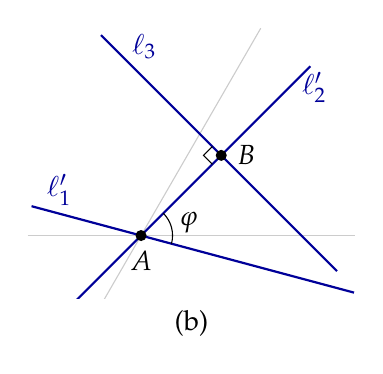
\begin{tikzpicture}[scale=0.8]
    \begin{scope}
        \clip (-1.8,-1.0) rectangle (3.4,3.3);
        \coordinate (A) at (0,0);
        \coordinate (B) at (45:1.8);
        \draw[gray!40] (180:1.8) -- (0:3.4);
        \draw[gray!40] (240:1.7) -- (60:3.8);
        \draw[mirror] (165:1.8) -- (-15:3.5);
        \draw[mirror] (225:1.6) -- (45:3.8);
        \draw[mirror] ($(B)+(135:2.7)$) -- ($(B)+(-45:2.6)$);
        \node[mirrorc] at (-1.3,0.72) {$\ell_1'$};
        \node[mirrorc] at (2.75,2.35) {$\ell_2'$};
        \node[mirrorc] at (0.05,3.0) {$\ell_3$};
        \draw ($(B)+(225:0.2)$) -- ($(B)+(225:0.2)+(135:0.2)$) -- ($(B)+(135:0.2)$);
        \draw (-15:0.5) arc (-15:45:0.5);
        \node at (15:0.78) {$\varphi$};
        \node[pt, label=below:{$A$}] at (A) {};
        \node[pt, label=right:{$B$}] at (B) {};
    \end{scope}
    \node at (0.8,-1.4) {(b)};
\end{tikzpicture}

\bigskip
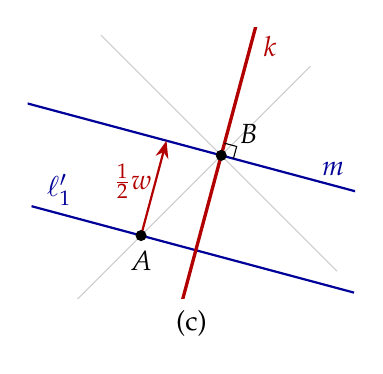
\begin{tikzpicture}[scale=0.8]
    \begin{scope}
        \clip (-1.8,-1.0) rectangle (3.4,3.3);
        \coordinate (A) at (0,0);
        \coordinate (B) at (45:1.8);
        \draw[gray!40] (225:1.6) -- (45:3.8);
        \draw[gray!40] ($(B)+(135:2.7)$) -- ($(B)+(-45:2.6)$);
        \draw[mirror] (165:1.8) -- (-15:3.5);
        \draw[mirror] ($(B)+(165:3.4)$) -- ($(B)+(-15:2.3)$);
        \draw[very thick, imgc] ($(B)+(255:2.5)$) -- ($(B)+(75:2.5)$);
        \draw ($(B)+(-15:0.2)$) -- ($(B)+(-15:0.2)+(75:0.2)$) -- ($(B)+(75:0.2)$);
        \node[mirrorc] at (-1.3,0.72) {$\ell_1'$};
        \node[mirrorc] at (3.05,1.05) {$m$};
        \node[imgc] at (2.05,3.0) {$k$};
        \draw[vec, imgc] (A) -- (75:1.559);
        \node[imgc] at ($(75:0.8)+(165:0.35)$) {$\tfrac12 w$};
        \node[pt, label=below:{$A$}] at (A) {};
        \node[pt, label={[label distance=1pt]15:{$B$}}] at (B) {};
    \end{scope}
    \node at (0.8,-1.4) {(c)};
\end{tikzpicture}
\hspace{1.2cm}
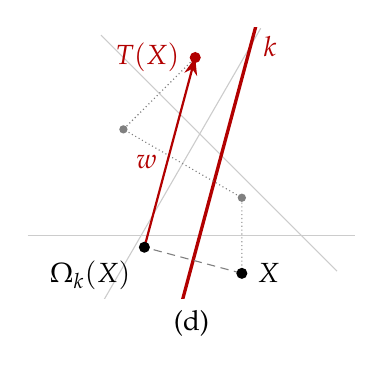
\begin{tikzpicture}[scale=0.8]
    \begin{scope}
        \clip (-1.8,-1.0) rectangle (3.4,3.3);
        \coordinate (A) at (0,0);
        \coordinate (B) at (45:1.8);
        \coordinate (X) at (1.6,-0.6);
        \coordinate (X1) at (1.6,0.6);
        \coordinate (X2) at (-0.2804,1.6856);
        \coordinate (TX) at (0.8599,2.8260);
        \coordinate (KX) at (0.0530,-0.1855);
        \draw[gray!40] (180:1.8) -- (0:3.4);
        \draw[gray!40] (240:1.7) -- (60:3.8);
        \draw[gray!40] ($(B)+(135:2.7)$) -- ($(B)+(-45:2.6)$);
        \draw[very thick, imgc] ($(B)+(255:2.5)$) -- ($(B)+(75:2.5)$);
        \draw[gray, densely dotted] (X) -- (X1) -- (X2) -- (TX);
        \node[circle, fill=gray, inner sep=0pt, minimum size=3pt] at (X1) {};
        \node[circle, fill=gray, inner sep=0pt, minimum size=3pt] at (X2) {};
        \draw[aux] (X) -- (KX);
        \draw[vec, imgc] (KX) -- (TX) node[pos=0.45, left] {$w$};
        \node[imgc] at (2.05,3.0) {$k$};
        \node[pt, label=right:{$X$}] at (X) {};
        \node[pt, label=below left:{$\Omega_k(X)$}] at (KX) {};
        \node[ipt, label={[imgc]left:{$T(X)$}}] at (TX) {};
    \end{scope}
    \node at (0.8,-1.4) {(d)};
\end{tikzpicture}
\captionof{figure}{(a) The three mirrors. (b) After Step 1. (c) After Steps 2 and 3. (d) The glide reflection.}\label{fig:general}
\end{plate}

\begin{problem}[When three reflections collapse to one]\label{p:collapse}
Let $\ell_1,\ell_2,\ell_3$ be lines, with concurrent and sharing a direction as in Problem~\ref{p:general}.\\
Show that $\Omega_{\ell_3}\circ\Omega_{\ell_2}\circ\Omega_{\ell_1}$ is a reflection $\Omega_{\ell_4}$ for some line $\ell_4$\\
if and only if the three lines are concurrent or share a direction.
\end{problem}

\begin{solution}
\leavevmode\\
Write $T=\Omega_{\ell_3}\circ\Omega_{\ell_2}\circ\Omega_{\ell_1}$.
\begin{enumerate}[leftmargin=2.5em]
    \item[($\Leftarrow$)] There are two cases.
    \begin{itemize}[nosep]
        \item \emph{Concurrent.} Let $P$ lie on all three lines.\\
        By Fact~\ref{f:anchor}(a) we can write $\ell_i=P+[v_i]$ with unit vectors $v_i$.\\
        Problem~\ref{p:three-concurrent} then gives a line $\ell_4$ through $P$ with $T=\Omega_{\ell_4}$.
        \item \emph{Common direction.} By Fact~\ref{f:anchor}(a) we can write $\ell_i=A_i+[v]$ with one unit $v$.\\
        Put $n=v^\perp$, $A_4=A_1+\ip{A_3-A_2}{n}n$ and $\ell_4=A_4+[v]$.\\
        Since $\ip{A_4-A_1}{n}=\ip{A_3-A_2}{n}$, Fact~\ref{f:parallel-mirrors} applied to both pairs gives
        \[
        \Omega_{\ell_4}\circ\Omega_{\ell_1}=T_{2\ip{A_3-A_2}{n}n}=\Omega_{\ell_3}\circ\Omega_{\ell_2}.
        \]
        Composing on the right with $\Omega_{\ell_1}$ and using Problem~\ref{p:bijection} gives $\Omega_{\ell_4}=T$.\\
        So $\ell_4$ is $\ell_1$ shifted by the gap from $\ell_2$ to $\ell_3$, the parallel analogue of Problem~\ref{p:three-concurrent}.
    \end{itemize}
    \item[($\Rightarrow$)] Suppose the lines are neither concurrent nor share a direction.\\
    By Problem~\ref{p:general}, $T$ is a glide reflection.\\
    So $T$ has no fixed point by Problem~\ref{p:glide-square}(b).\\
    But every reflection $\Omega_\ell$ fixes the points of $\ell$ (Problem~\ref{p:fixed}).\\
    Hence $T$ is not a reflection. \qedhere
\end{enumerate}
\end{solution}

\begin{remark}
So a composition of three reflections is always a reflection or a glide reflection.\\
The position of the mirrors tells which (Figure~\ref{fig:collapse}).
\end{remark}

\begin{plate}
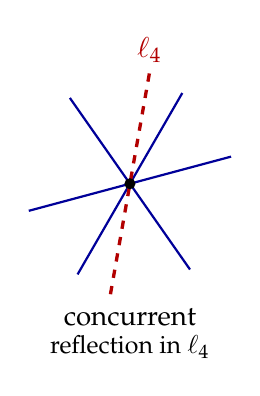
\begin{tikzpicture}[scale=0.95]
    \draw[mirror] (195:1.4) -- (15:1.4);
    \draw[mirror] (240:1.4) -- (60:1.4);
    \draw[mirror] (305:1.4) -- (125:1.4);
    \draw[very thick, imgc, dashed] (260:1.5) -- (80:1.5) node[above] {$\ell_4$};
    \node[pt] at (0,0) {};
    \node[align=center] at (0,-2.0) {concurrent\\[-2pt] \small reflection in $\ell_4$};
\end{tikzpicture}
\hspace{0.8cm}
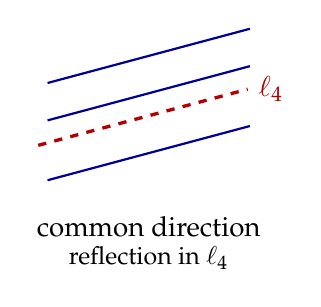
\begin{tikzpicture}[scale=0.95]
    \foreach \y in {-0.8,0,0.5} {
        \draw[mirror] ($(0,\y)+(195:1.4)$) -- ($(0,\y)+(15:1.4)$);
    }
    \draw[very thick, imgc, dashed] ($(-0.125,-0.3335)+(195:1.4)$) -- ($(-0.125,-0.3335)+(15:1.5)$) node[right] {$\ell_4$};
    \node[align=center] at (0,-2.0) {common direction\\[-2pt] \small reflection in $\ell_4$};
\end{tikzpicture}
\hspace{0.8cm}
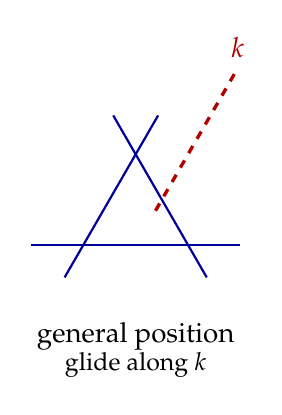
\begin{tikzpicture}[scale=0.95]
    \draw[mirror] (-1.2,-0.6) -- (1.6,-0.6);
    \draw[mirror] ($(-0.5,-0.6)+(240:0.5)$) -- ($(-0.5,-0.6)+(60:2.0)$);
    \draw[mirror] ($(0.9,-0.6)+(300:0.5)$) -- ($(0.9,-0.6)+(120:2.0)$);
    \draw[very thick, imgc, dashed] ($(1.1147,0.9843)+(240:1.3)$) -- ($(1.1147,0.9843)+(60:0.9)$) node[above] {$k$};
    \node[align=center] at (0.2,-2.0) {general position\\[-2pt] \small glide along $k$};
\end{tikzpicture}
\captionof{figure}{The three cases, with the resulting mirror $\ell_4$ or glide axis $k$ in red.}\label{fig:collapse}
\end{plate}

\newpage
\section*{6. Isometries and Lines}

\begin{problem}[Isometries carry lines onto lines]\label{p:lines-to-lines}
Let $T\colon\E\to\E$ be an isometry, so $d(T(X),T(Y))=d(X,Y)$ for all points $X$ and $Y$.\\
Let $\ell$ be a line.
\begin{enumerate}
    \item Show that $T(\ell)$ is contained in a line.
    \item Show that $T(\ell)$ is a line.\\
    More precisely, if $A\neq B$ are points of $\ell$, show that for every $s\in\R$
    \[
    T\bigl(A+s(B-A)\bigr)=T(A)+s\bigl(T(B)-T(A)\bigr).
    \]
\end{enumerate}
\end{problem}

\begin{solution}
\leavevmode
\begin{enumerate}
    \item Write $\ell=P+[v]$ with $\abs{v}=1$ and let $Q=P+v^\perp$.\\
    Since $\ip{Q-P}{v^\perp}=1\neq0$, we have $Q\notin\ell$ by Problem~\ref{p:normal}(b).\\
    Put $Q'=\Omega_\ell(Q)$. Then $Q'\neq Q$ by Problem~\ref{p:fixed}, and Problem~\ref{p:equidistant} gives
    \[
    \ell=\{X\in\E \mid d(X,Q)=d(X,Q')\}.
    \]
    For $X\in\ell$, since $T$ preserves distances
    \[
    d(T(X),T(Q))=d(X,Q)=d(X,Q')=d(T(X),T(Q')).
    \]
    As $T$ is injective, $T(Q)\neq T(Q')$. So by Corollary~\ref{c:bisector}, $T(\ell)$ lies in the line
    \[
    m=\{Y\in\E \mid d(Y,T(Q))=d(Y,T(Q'))\}.
    \]
    In Figure~\ref{fig:lines-to-lines}, $T$ keeps the equal distances from $X$ to $Q$ and to $Q'$.
    \item Let $A\neq B$ be points of $\ell$, and put $A'=T(A)$ and $B'=T(B)$.\\
    Then $A'\neq B'$ because $T$ is injective, and both lie on $m$ by (a).\\
    By Problem~\ref{p:two-points}, $\ell=A+[B-A]$ and $m=A'+[B'-A']$.\\
    Put $\delta=\abs{B-A}$. Then $\delta>0$, and $\delta=\abs{B'-A'}$ since $T$ is an isometry.\\
    Take $X=A+s(B-A)$ in $\ell$. By (a), $T(X)=A'+\lambda(B'-A')$ for some $\lambda\in\R$.\\
    Comparing distances to $A'$ and to $B'$ gives
    \begin{align*}
    \abs{\lambda}\delta &= d(T(X),A')=d(X,A)=\abs{s}\delta\\
    \abs{\lambda-1}\delta &= d(T(X),B')=d(X,B)=\abs{s-1}\delta.
    \end{align*}
    Hence $\lambda^2=s^2$ and $(\lambda-1)^2=(s-1)^2$.\\
    Subtracting gives $-2\lambda+1=-2s+1$, so $\lambda=s$, as Problem~\ref{p:parameter} predicts. Therefore
    \[
    T\bigl(A+s(B-A)\bigr)=A'+s(B'-A') \qquad\text{for all } s\in\R.
    \]
    As $s$ runs over $\R$, the two sides run over $T(\ell)$ and $m$, so $T(\ell)=m$. \qedhere
\end{enumerate}
\end{solution}

\begin{remark}
With $s\in[0,1]$, $T$ maps points between $A$ and $B$ onto points between $A'$ and $B'$.
\end{remark}

\begin{plate}
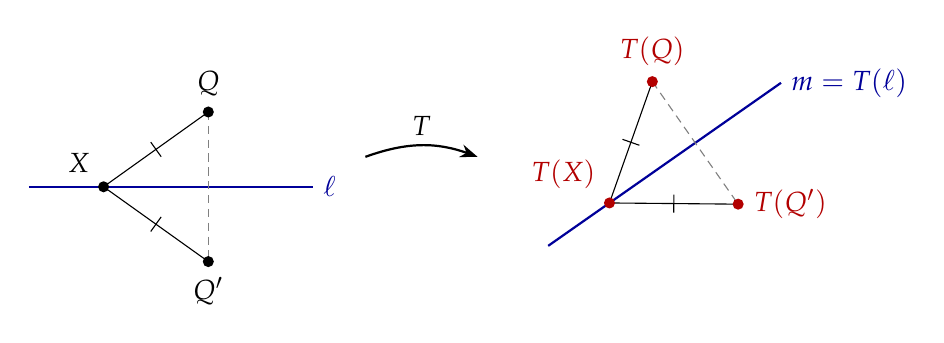
\begin{tikzpicture}[scale=0.95]
    \begin{scope}
        \coordinate (Q) at (0.5,1.0);
        \coordinate (Qr) at (0.5,-1.0);
        \coordinate (X) at (-0.9,0);
        \draw[mirror] (-1.9,0) -- (1.9,0) node[right] {$\ell$};
        \draw[aux] (Q) -- (Qr);
        \draw (X) -- (Q);
        \draw (X) -- (Qr);
        \eqtick{X}{Q}
        \eqtick{X}{Qr}
        \node[pt, label=above:{$Q$}] at (Q) {};
        \node[pt, label=below:{$Q'$}] at (Qr) {};
        \node[pt, label=above left:{$X$}] at (X) {};
    \end{scope}
    \draw[->, thick] (2.6,0.4) to[bend left=20] node[above] {$T$} (4.1,0.4);
    \begin{scope}[shift={(6.6,0.3)}, rotate=35]
        \coordinate (TQ) at (0.5,1.0);
        \coordinate (TQr) at (0.5,-1.0);
        \coordinate (TX) at (-0.9,0);
        \draw[mirror] (-1.9,0) -- (1.9,0) node[right] {$m=T(\ell)$};
        \draw[aux] (TQ) -- (TQr);
        \draw (TX) -- (TQ);
        \draw (TX) -- (TQr);
        \eqtick{TX}{TQ}
        \eqtick{TX}{TQr}
        \node[ipt, label={[imgc]above:{$T(Q)$}}] at (TQ) {};
        \node[ipt, label={[imgc]right:{$T(Q')$}}] at (TQr) {};
        \node[ipt, label={[imgc]above left:{$T(X)$}}] at (TX) {};
    \end{scope}
\end{tikzpicture}
\captionof{figure}{A line $\ell$ with points $X$, $Q$ and $Q'=\Omega_\ell(Q)$, and their images under $T$.}\label{fig:lines-to-lines}
\end{plate}

\end{document}
